% Sample LaTeX file for creating a paper in the Morgan Kaufmannn two
% column, 8 1/2 by 11 inch proceedings format.

\documentclass[]{article}
\usepackage{proceed2e}
\usepackage{hyperref}
\usepackage{url}
\usepackage{amsmath}
\usepackage{graphicx}
\usepackage{bm}
\usepackage{hyperref}
\usepackage{natbib}
\usepackage{latexsym,amsbsy,amssymb,color,xspace, booktabs}

% genereal purpose macros here
\newcommand{\marg}{\marginpar}
\newcommand{\todo}[1]{{\color{red}{TODO: #1}}}
\newcommand{\commentOut}[1]{} 
\newcommand{\add}[1]{\textcolor{red}{#1}} % To highligh modified text

% abbreviations
\newcommand{\etal}{et al.\xspace}
\newcommand{\ie}{i.e.\xspace}
\newcommand{\eg}{e.g.\xspace}
\newcommand{\Ie}{I.e.\xspace}



% Matrices and vectors 
\newcommand{\mat}[1]{\mathbf{#1}}
\renewcommand{\vec}[1]{ \mathbf{#1} } % math bold
\newcommand{\vecS}[1]{\boldsymbol{ #1 }  } % this for boldsymbols
\newcommand{\vecentry}[2]{{\mathrm #1_{#2}}}
\newcommand{\matentry}[3]{{\mathrm #1_{#2,#3}}}
\newcommand{\matcol}[2]{\mat{#1}_{\cdot #2}}
\newcommand{\matrow}[2]{\mat{#1}_{#2 \cdot}}

 % Matrices here
 \newcommand{\A}{\mat{A}}
\newcommand{\B}{\mat{B}}
\newcommand{\C}{\mat{C}}
\newcommand{\D}{\mat{D}}
\newcommand{\F}{\mat{F}}
\newcommand{\G}{\mat{G}}
\newcommand{\I}{\mat{I}}
\renewcommand{\L}{\mat{L}}
\newcommand{\X}{\mat{X}}
\newcommand{\W}{\mat{W}}
\newcommand{\Y}{\mat{Y}}
\newcommand{\Z}{\mat{Z}}
\renewcommand{\S}{\mat{S}}
\newcommand{\K}{\mat{K}}
\newcommand{\U}{\mat{U}}

% Vectors here
\newcommand{\f}{\vec{f}}
\newcommand{\g}{\vec{g}}
\newcommand{\h}{\vec{h}}
\newcommand{\m}{\vec{m}}
\renewcommand{\t}{\vec{t}}
\renewcommand{\u}{\vec{u}}
\newcommand{\w}{\vec{w}}
\newcommand{\x}{\vec{x}}
\newcommand{\y}{\vec{y}}
\newcommand{\z}{\vec{z}}

 % Vectorial greek letters
  \newcommand{\vecmu}{\vecS{\mu}}
 \newcommand{\vectheta}{\vecS{\theta}}
 \newcommand{\vecalpha}{\vecS{\alpha}}
 \newcommand{\vecphi}{\vecS{\phi}}
 \newcommand{\veceta}{\vecS{\eta}}
 \newcommand{\vecepsilon}{\vecS{\epsilon}} 
 
% caligraphic alphabet
\newcommand{\calA}{\mathcal{A}}
\newcommand{\calC}{\mathcal{C}}
\newcommand{\calD}{\mathcal{D}} 
\newcommand{\calL}{\mathcal{L}}
\newcommand{\calM}{\mathcal{M}}
\newcommand{\calT}{\mathcal{T}}
\newcommand{\calU}{\mathcal{U}}
\newcommand{\calX}{\mathcal{X}}
\newcommand{\calF}{\mathcal{F}}
\newcommand{\calE}{\mathcal{E}}
\newcommand{\calH}{\mathcal{H}}
\newcommand{\calI}{\mathcal{I}}
\newcommand{\calS}{\mathcal{S}}
\newcommand{\calY}{\mathcal{Y}}
\newcommand{\calO}{\mathcal{O}}
\newcommand{\calQ}{\mathcal{Q}}
\newcommand{\calR}{\mathcal{R}}
\newcommand{\calV}{\mathcal{V}}


% blackboard alphabet 
\newcommand{\setR}{\mathbb{R}}
\newcommand{\setE}{\mathbb{E}}
\newcommand{\setV}{\mathbb{V}}
\newcommand{\setI}{\mathbb{I}}
\newcommand{\setX}{\mathbb{X}}
\newcommand{\setT}{\mathbb{T}}



% Useful math operators
\newcommand{\Sum}{{\displaystyle \sum}}
\DeclareMathOperator{\vect}{vec}
\DeclareMathOperator{\diag}{diag}
\DeclareMathOperator*{\argmax}{argmax}                 
\DeclareMathOperator*{\argmin}{argmin}                 
\providecommand{\abs}[1]{\lvert#1\rvert}
\providecommand{\norm}[1]{\lVert#1\rVert}
\newcommand{\notp}[1]{\stackrel{\neg}{#1}} % symbol for not present


% matrix products
\newcommand{\kron}{\otimes}
\newcommand{\hada}{\bullet}

% statistics
\newcommand{\expectation}{\mathbb{E}}
\newcommand{\Eb}[1]{\left\langle #1 \right\rangle} % Expectation in angle brackets
\newcommand{\variance}{\mathbb{V}}
\newcommand{\Normal}{\mathcal{N}}  
\newcommand{\avg}[1]{\overline{#1}}
\newcommand{\KL}{\text{KL}}

% GP things
\newcommand{\GP}{\mathcal{GP}}
\newcommand{\kernel}{\kappa}

% Other maths
\newcommand{\deriv}[2]{\frac{\partial{#1}}{\partial{#2}}}
\newcommand{\trace}{\mbox{ \rm tr }}
\renewcommand{\det}[1]{\lvert#1\rvert}
\newcommand{\defeq}{\stackrel{\text{\tiny def}}{=}}
\newcommand{\idx}{\mathcal{I}}
\newcommand{\T}{\text{T}}
\newcommand{\mth}{\mathrm{th}} 


\newcommand{\bigO}{\calO}
\newcommand{\define}{\overset{\Delta}{=}}




















\newcommand{\gprnmf}{{\sc{gprn-mf}}}
\newcommand{\gprnnpv}{{\sc{gprn-npv}}}
\newcommand{\igp}{{\sc{igp}}}
\newcommand{\npv}[1]{{\sc{npv#1}}}
\newcommand{\fitc}{{\sc{fitc}}}

\newcommand{\vecu}{\vec{u}}
\newcommand{\vecf}{\vec{f}}
\newcommand{\vecy}{\vec{y}}
\newcommand{\vecw}{\vec{w}}
\newcommand{\vecfhat}{\hat{\vec{f}}}
\newcommand{\kernelf}{\kernel_{f}}
\newcommand{\kernelw}{\kernel_{w}}
\newcommand{\vecthetaf}{\vectheta_{f}}
\newcommand{\vecthetaw}{\vectheta_{w}}
\newcommand{\sigmaf}{\sigma_{f}}
\newcommand{\sigmay}{\sigma_{y}}
\newcommand{\Cu}{\mat{\C}_{u}}
\newcommand{\elbo}{\calL} % Evidence lower bound
\newcommand{\entropy}{\calH}
\newcommand{\p}{P} % Number of outputs
\newcommand{\q}{Q} % Number of latent functions
\newcommand{\vecfj}{\vec{f}_{j}}
\newcommand{\vecmufj}{\vecS{\mu}_{\text{f}_{\text{j}}}}
\newcommand{\vecmufk}{\vecS{\mu}_{\text{f}_{\text{k}}}}
\newcommand{\Sigmafj}{\mat{\Sigma}_{\text{f}_{\text{j}}}}
\newcommand{\vecwij}{\vec{w}_{ij}}
\newcommand{\vecmuwij}{\vecS{\mu}_{\text{w}_{\text{ij}}}}
\newcommand{\vecmuwik}{\vecS{\mu}_{\text{w}_{\text{ik}}}}
\newcommand{\Sigmawij}{\mat{\Sigma}_{\text{w}_{\text{ij}}}}
\newcommand{\matY}{\mat{Y}}
\newcommand{\vecmufn}{\vecS{\nu}_{\text{f}_{\text{n}}}} % These are for data structures for a fixed observation
\newcommand{\matMuwn}{\mat{\Omega}_{\text{w}_{\text{n}}}} % These are for data structures for a fixed observation
\newcommand{\Kf}{\mat{K}_{f}}
\newcommand{\Kw}{\mat{K}_{w}}
\newcommand{\Kfinv}{\mat{K}_{f}^{-1}}
\newcommand{\Kwinv}{\mat{K}_{w}^{-1}}

\newcommand{\vecyn}{\matcol{Y}{n}^{T}}
\newcommand{\sigmak}{\sigma_{k}}
\newcommand{\vecystar}{\vec{y}^*}
\newcommand{\vecxstar}{\vec{x}^*}
\newcommand{\vecWstar}{\vec{W}^*}
\newcommand{\vecfstar}{\vec{f}^*}
\newcommand{\der}{\mathrm{d}}
\newcommand{\vecmuw}{\vecS{\mu}_{\textbf{w}}}
\newcommand{\vecmuf}{\vecS{\mu}_{\textbf{f}}}
\newcommand{\Kwstar}{\Kw^*}
\newcommand{\Kfstar}{\Kf^*}

\newcommand{\sigmanoise}{\sigma_{\text{n}}}
\newcommand{\sigmoid}{\text{sig}}
\newcommand{\vf}{\vec{f}}
\newcommand{\vy}{\vec{y}}
\newcommand{\vu}{\vec{u}}
\newcommand{\vz}{\vec{z}}
\newcommand{\vx}{\vec{x}}
\newcommand{\vw}{\vec{w}}
\newcommand{\vg}{\vec{g}}
\newcommand{\vh}{\vec{h}}
\newcommand{\vm}{\vec{m}}
\newcommand{\matU}{\mat{U}}
\newcommand{\matX}{\mat{X}}
\newcommand{\Xu}{\mat{X}_u}
\newcommand{\bs}{\boldsymbol}
\newcommand{\xstar}{x_*}
\newcommand{\vxstar}{\vx_*}
\newcommand{\ystar}{y_*}
\newcommand{\zstar}{z_*}
\newcommand{\vfstar}{\vf_*}
\newcommand{\fstar}{f_*}
\newcommand{\Xuk}{\Xu^{(k)}}
\newcommand{\Kab}[2]{\mat{K}_{\vec{#1},\vec{#2}}}

% model specification
\newcommand{\BigMu}{\bs{\mu}}
\newcommand{\BigSigma}{\mat{\Sigma}}
\newcommand{\Mu}{\BigMu}
\newcommand{\Muk}{\bs{\mu}_k}
\newcommand{\Sigmak}{\mat{\Sigma}_k}
\newcommand{\hatMuk}{\bs{\hat \mu}_k}
\newcommand{\hatSigmak}{\mat{\hat \Sigma}_k}
\newcommand{\hatMukprime}{\bs{\hat \mu}_{k'}}
\newcommand{\hatSigmakprime}{\mat{\hat \Sigma}_{k'}}
\newcommand{\thetak}{\bs{\theta}_k}
\newcommand{\BigTheta}{\bs{\theta}}
\newcommand{\bsigma}{\bs{\sigma}}
\newcommand{\map}{\text{\sc{map}}}
\newcommand{\zmap}{\vz_\text{\sc{map}}}
\newcommand{\fuk}{\vec{g}_k}
\newcommand{\fu}{\vec{g}}
\newcommand{\kernelk}{k^{\BigTheta_k}}
\newcommand{\matUk}{\mat{U}_k}
\newcommand{\matXk}{\mat{X}_k}
\newcommand{\Lambdak}{\Lambda^{\BigTheta_k}}
\newcommand{\matK}{\mat{K}}
\newcommand{\matLambdak}{\mat{\Lambda}_k}

% variational inference
\newcommand{\Mufk}{\BigMu_k}
\newcommand{\Sigmafk}{\BigSigma_k}
\newcommand{\Kuk}{\matK^{(k)}_{\vu,\vu}}
\newcommand{\Psik}{\mat{\Psi}_k}
\newcommand{\Gammak}{\mat{\Gamma}_k}


\title{Collaborative Multioutput Gaussian Processes}

\author{} % LEAVE BLANK FOR ORIGINAL SUBMISSION.
          % UAI  reviewing is double-blind.

% The author names and affiliations should appear only in the accepted paper.
%
%\author{ {\bf Harry Q.~Bovik\thanks{Footnote for author to give an
%alternate address.}} \\
%Computer Science Dept. \\
%Cranberry University\\
%Pittsburgh, PA 15213 \\
%\And
%{\bf Coauthor}  \\
%Affiliation          \\
%Address \\
%\And
%{\bf Coauthor}   \\
%Affiliation \\
%Address    \\
%(if needed)\\
%}

\begin{document}

\maketitle

\begin{abstract}
The Abstract paragraph 
\end{abstract}

\section{INTRODUCTION}
% Gaussian processes are good for bayesian regression, Very flexible in multi-output settings, for e.g. bonilla, alvarez, wilson
Gaussian process models  \citep[GPs,][]{rasmussen-williams-book}  are a popular choice in 
Bayesian regression due to their ability to capture complex dependencies and non-linearities in data.
In particular, when having multiple outputs or tasks they have proved effective in modeling 
the dependencies between the tasks  and  they have been shown to outperform competitive baselines and 
single output learners  \citep{bonilla-et-al-nips-08,teh-et-al-aistats-05,alvarez-lawrence-nips-08,wilson-et-al-icml-12}.
% However they are costly
However, the prohibitive cost of performing exact inference in  GP models severely hinders 
their application to  large scale multi-output problems. For example, na\"{i}ve inference 
in a fully coupled Gaussian process model over $P$  outputs and $N$ data-points can have 
a complexity of $\calO(N^3P^3)$  and $\calO(N^2P^2)$ in time and memory, respectively.


% Motivating example is good
A motivating  example of a large scale multi-output application 
is the tracking of  movements of a robot arm using 2 or more joint torques. 
If one of the robot motors malfunctions and fails to record a torque, data collected from the 
other motors may be used to infer the missing torque values.
However, taking 100 measurements per second already results in a total of over 40,000 data points 
per torque in just 7 minutes.
Clearly this problem is well beyond the capabilities  of conventional multiple output GPs.
Building  multi-output GP models that can learn correlated tasks at the scale of 
these types of problems  is thus the main focus of this paper.

% Tranditional approaches in single output setting, based e..g. on inducing points are not good enough 
In the single output setting previous attempts to scale up  GP inference 
resort to approximate inference. Most  approximation techniques 
 can be understood 
within a single probabilistic framework that uses a set of \emph{inducing points}  in order to 
obtain an approximate process (or a low-rank approximate covariance) over which inference can be 
performed more efficiently \citep{quinonero2005unifying}. These models have been referred 
to in the literature as sparse models. 
Nevertheless, straightforward application of such approximate techniques will yield a computational 
cost of at least $\calO(PNM^2)$ in time and  $\calO(PNM)$ in memory, where 
$M$ is the number of inducing points. This high complexity still prevents us from applying GP models 
to  large scale multi-output problems.

% Useful observations
In this work we approach the challenge of building scalable multi-output Gaussian process models  
based on the following observations.
Firstly, \emph{inducing variables} are the key catalyst
for achieving sparsity and dealing with large scale problems in Gaussian process models.
In particular, they capture the \emph{sufficient statistics} of a dataset allowing the construction of sparse 
processes that can approximate arbitrarily well the exact GP model \citep{titsias2009variational}.
Secondly, the use of global latent variables (such as the inducing points) allows us to 
induce dependencies in a highly correlated model efficiently. 
This observation is exploited in \cite{hensmangaussian} for single output GP regression models 
where, by explicitly representing a distribution over the inducing variables, stochastic variational inference 
can be used to work with millions of data points.
Finally, the key to multi-output and multi-task learning is to model dependencies between the outputs  
based on realistic assumptions of what can be shared across the tasks. It turns out that 
sharing  ``sparsity structure'' can not only be a reasonable assumption but also a crucial component
when modeling dependencies between different related tasks.


% Our approach starts from mixing latent process
% having inducing points for sparsity
% sharing inducing points across the latent process
Based on these observations, we propose the collaborative multi-output Gaussian Process (COGP) model 
where each output is a weighted combination of sparse latent processes.
 Each latent process has its own set of inducing points that sufficiently encapsulates the process signal and characteristics.
Correlations among the outputs are fostered via sharing of multiple inducing point sets 
which in turn create a medium through which joint inference happens efficiently.
% exploit stochastic variational inference
In particular, we derive a variational lower bound of the model evidence that decomposes across 
inputs and outputs. 
This decomposition makes possible the application of stochastic variational inference, 
thus allowing the model to handle a large number of observations per output and a large number of outputs.
Furthermore, learning of all  the  parameters in the model, including
kernel hyperparameters and inducing inputs, can be done in a single stochastic optimization framework.

We analyze our multi-out model on a toy problem  where the inducing variables are shown to be 
conducive to the sharing of information between two related tasks. 
Additionally, we  evaluate  our model on two moderate-sized datasets in which we show that it
can outperform previous non-scalable multi-output approaches as well as single output baselines.
Finally, on a  large scale experiment regarding the learning of robot inverse dynamics we show 
the substantial benefits of collaborative learning provided by our model.
  
% Experiments and summary of results
%The rest of the paper is organized as follows.
%We give description of the model in Section \ref{sec:model}, followed by the inference procedure in Section \ref{sec:inference}. 
%Section \ref{sec:experiments} presents empirical evaluation.
%We conclude with some discussion in Section \ref{sec:discussion}.

% Some citations that can be brought back somewhere
\paragraph{Related work.}
Most GP-based multi-output models create correlated outputs by mixing a set of independent latent processes.
The mixing can be a linear combination with fixed coefficients \citep[see e.g.][]{teh-et-al-aistats-05,bonilla-et-al-nips-08}. This is known in the geostatistics community as  the ``linear model of coregionalization'' \citep{goovaerts1997geostatistics}.
Such models may also be reformulated in a common Bayesian framework, for example by placing a spike and slab prior over the coefficients \citep{titsias2011spike}.
More complex dependencies can be induced by using 
 input-dependent coefficients \citep{wilson-et-al-icml-12,nguyen2013efficient}  or convolving processes \citep{boyle-frean-nips-05,alvarez-lawrence-nips-08,alvarez2010efficient}.
 
While we also use the mixing construction, the key difference in our model is the role of inducing variables.
In particular, when used in previous models to reduce the computational costs \citep[see e.g.][]{alvarez-lawrence-nips-08,alvarez2010efficient}, the inducing points are integrated out or collapsed. 
In contrast, our model maintains an explicit representation of the posterior over the inducing variables that is learned using data from all outputs.
This explicit representation  facilitates scalable learning in a similar fashion to 
the approach in \citet{hensmangaussian}, making it applicable to very large datasets. 













\section{MODEL DESCRIPTION}
Before diving into technical details of the model specification, 
we discuss the modeling philosophy behind our collaborative multi-output Gaussian processes.
To learn the outputs jointly, we need a mechanism through which information can be transferred among the outputs.
This is achieved in the model by allowing the outputs to share multiple sets of inducing variables, 
each of which captures a different pattern common to the outputs.
These variables  play a double pivotal role in the model: they collaboratively share  information 
across the outputs and  provide \emph{sufficient statistics}  so as to induce sparse processes. 

\newcommand{\Zj}{\Z_j}
\newcommand{\Zhi}{\Z^h_i}
Consider the joint regression of $P$ tasks with inputs $\X = \{\x_n \in \calR^D\}_{n=1}^N$ and outputs $\y = \{\y_i\}_{i=1}^P$ where $\y_i = \{y_{in}\}_{n=1}^N$.
We  model each output as a weighted combination of $Q$ shared latent functions $\{ g_{j}\}_{j=1}^{Q}$, plus an individual latent 
function $\{ h_{i}\}_{i=1}^{P}$ unique to that output for greater flexibility.
The $Q$ shared functions have independent Gaussian process priors  $g_j(\x) \sim \GP(0, k_j(\cdot,\cdot))$. %, with $j= 1, \ldots Q$.
Similarly, each individual function of an output also has GP prior, i.e.~$h_i(\x) \sim \GP(0, k^h_i(\cdot,\cdot))$. %with $i=1 ,\ldots P$.


As we want to sparsify these processes, 
we introduce the set of \emph{shared inducing variables} $\u_j$ for  each $g_j(\x)$, i.e. $\u_j$ contains the values of 
$g_j(\x)$ at the inducing inputs $\Z_j$. Likewise, we have 
individual inducing variables corresponding to each  $h_i(\x)$,  which we denote with with $\v_i$ and their 
corresponding inducing inputs $\Zhi$.
%
The inducing inputs lie in the same space as the inputs $\X$.
% which should be apparent since their corresponding values come from the processes defined on the input space.
For convenience, we  assume all processes have the same number of inducing points, $M$, however we emphasize that this is not
 imposed in practice.

% information is transfered via the inducing variables

We denote the collective variables: $\g = \{\g_j\}$, $\h = \{\h_i \}$, $\u = \{\u_j\}$, $\v = \{\v_i\}$, $\Z = \{\Zj\}$, and $\Z^h = \{\Zhi \}$ where $\g_j = \{g_j(\x_n)\}$, $\h_i = \{h_i(\x_n)\}$. 
Note that we reserve subscript $i$ for indexing the outputs and their corresponding individual processes ($i = 1 \hdots P$), $j$ for the latent processes ($j = 1 \hdots Q$), and $n$ for the inputs ($n = 1 \hdots N$).
%
\subsection{PRIOR MODEL}
From the definition of the GPs and the conditional independence of the processes given the inducing variables, 
the \emph{prior} of the multi-output model can be written as:
\begin{align}
\label{eq:gu}
p(\g | \u) &= \prod_{j=1}^Q p(\g_j | \u_j) = \prod_{j=1}^Q \Normal(\g_j; \BigMu_j, \tilde{\K}_j )\\
\label{eq:u}
p(\u) &= \prod_{j=1}^Q p(\u_j) = \prod_{j=1}^Q \Normal(\u_j; \vec{0}, k(\Zj, \Zj)) \\
\label{eq:hv}
p(\h | \v) &= \prod_{i=1}^P p(\h_i | \v_i) = \prod_{i=1}^P \Normal(\h_i; \BigMu^h_i, \tilde{\K}^h_i)\\
\label{eq:v}
p(\v) &= \prod_{i=1}^P p(\v_i) = \prod_{i=1}^P \Normal(\v_i; \vec{0}, k(\Zhi, \Zhi)),
\end{align}
where the corresponding means and covariances of the Gaussians are given by:
\begin{align}
 \BigMu_j &= k(\X,\Zj)k(\Zj,\Zj)^{-1}\u_j \\
\BigMu^h_i &= k(\X,\Zhi)k(\Zhi,\Zhi)^{-1}\v_i \\
\tilde{\K}_j &= k_j(\X,\X) - k(\X,\Zj)k(\Zj,\Zj)^{-1}k(\Zj,\X) \\
\tilde{\K}^h_i &= k^h_i(\X,\X) - k(\X,\Zhi)k(\Zhi,\Zhi)^{-1}k(\Zhi,\X).
\end{align}
In the equations and hereafter, we omit the subscripts $j,h,i$ from the kernels $k_j(\cdot,\cdot)$ and $k^h_i(\cdot,\cdot)$ when it is clear from the parameters inside the parentheses which covariance function is in action.
Here, equations \ref{eq:u} and \ref{eq:v} follow directly from the properties of GPs, while the expressions for $p(\g|\u)$ and $p(\h|\v)$ (eq. \ref{eq:gu} and \ref{eq:hv}) come from the conditionals of the multivariate Gaussian distributions.
Instead of writing the joint priors $p(\g,\u)$ and $p(\h,\v)$, the above equivalent equations are given to emphasize the important role of the inducing variables in the model.
%
\subsection{LIKELIHOOD MODEL}
As mentioned above, we assume that  observations for each output 
are  (noisy) linear combinations of the $Q$ latent functions $g_{j}(\vec{x})$ plus
an independent function $h_{i}(\vec{x})$. Hence we have that the likelihood 
with standard iid Gaussian noise is given by:
\begin{align}
p(\y | \g, \h ) = \prod_{i=1}^P \prod_{n=1}^N \Normal( y_{in} ; \sum_{j=1}^Q w_{ij} g_j(\x_n) + h_i(\x_n), \beta_i^{-1}),
\end{align}
where $w_{ij}$ are the corresponding weights and $\beta_i$ is the precision of each Gaussian.
%which says that $y_{in}$ is a linear combination of the latent functions with weight $w_{ij}$ for the $j$th shared latent process plus a contribution from the individual process $h_i$.
As the latent values $\g$ are specified conditioned on the inducing variables $\u$, this construction implies that each output is a weighted combination of the inducing values.
We note that if $\u$ and $\v$ are marginalized out, we obtain the semiparametric latent factor model \citep{teh-et-al-aistats-05}.
However, doing so is against the purpose of our model which encourages sharing of outputs via the inducing variables.
Furthermore, as we shall see in the next section, explicit representation of these variables is fundamental to scalable inference of the model.

%\textbf{Augmented sparse GPs}
%Toward scalable modeling, we replace standard GPs with sparse GPs augmented with \textit{different} set of inducing inputs.
%This adds much flexibility to the model as each of the shared process $g_j(\x)$ can model a different pattern in the data with its own covariance function and inducing inputs. The roles of $g_j(\x)$ and $h_i(\x)$ can be quite different, so it is necessary that each has its own inducing inputs.
%Furthermore, $g_j(\x)$ can be seen as a \textit{global} function operating on the entire input space (of all output dimensions), while each $h_i(\x)$ operates only on the inputs of the $i$-th output, which can be a subspace of the input.


\subsection{THIS SHOULD BE CAP}

\section{INFERENCE}
%\subsection{Variational Inference in Sparse GPs Revisited}
%
%In this section we review inference in sparse GPs (as presented in Titsias).
%The posterior in an augmented model is $p(\f, \u | \y) = p(\f | \u, \y) p(\u | \y)$.
%The key property of such augmented GPs  is the notion of \textit{sufficient statistics}: given the inducing points $\u$, the latent values $\f$ are independent with any other set of latent values (e.g. the test set).
%In the optimal setting when $\u$ is the sufficient statistics of $\f$, it should hold that $p(\f | \u, \y) = p(\f | \u)$ as $\y$ is only the noisy version of $\f$.
%This leads to choosing a variational approximation of the posterior which factorizes as $q(\f, \u | \y) = p(\f | \u) q(\u | \y)$.
%Since the conditional $p(\f | \u)$ is known, variational inference becomes learning an optimal posterior $q(\u | \y)$ only. \\
%
We approximate the posterior over the latent variables $\vec{g}, \vec{h}, \vec{u}, \vec{v}$ given observations $\vec{y}$ using variational inference \citep{jordan-variational-99}.
In section \ref{sec:variationalLowerBound} we derive a lower bound of the marginal likelihood which has the key property of factorizing over the data points and outputs. Section \ref{sec:svi}  takes advantage of this factorization to 
derive stochastic variational inference, allowing the model to scale to very large datasets.
Section \ref{sec:complexity} compares the complexity of the model with previous multi-output methods.

\subsection{VARIATIONAL LOWER BOUND \label{sec:variationalLowerBound}}
\newcommand{\ug}{\u_g}
\newcommand{\uh}{\u^h}
\newcommand{\mgj}{\m_j}
\newcommand{\mhi}{\m^h_i}
\newcommand{\Sgj}{\S_j}
\newcommand{\Shi}{\S^h_i}
In variational inference, we find the ``closest'' approximate distribution to the true posterior in terms of the $\KL$ divergence.
We first observe that the true posterior distribution can be written as:
\begin{align}
p(\g, \h, \u, \v | \y) = p(\g | \u, \y) p(\h | \v, \y) p(\u, \v | \y).
\end{align}
Here we recall the modeling assumption that each set of  inducing variables is the sufficient statistics of the corresponding latent process. 
This motivates replacing the true posteriors over $\g$ and $\h$ with their conditional distributions given the inducing variables, leading to a distribution of the form:
\begin{align}
q(\g, \h, \u, \v | \y)
= p(\g|\u) p(\h|\v) q(\u,\v),
\end{align}
with
\begin{align}
q(\u,\v) &= \prod_{j=1}^Q \underbrace{\Normal(\u_j; \mgj, \Sgj)}_{q(\u_j)} \prod_{i=1}^P  \underbrace{\Normal(\v_i; \mhi, \Shi)}_{q(\v_i)}.
\end{align}
This technique has been used by \citet{titsias2009variational} and \citet{hensmangaussian} 
to derive variational inference algorithms for the single output case.
Since the conditionals $p(\g | \u)$ and $p(\h | \v)$ are known (Equations \eqref{eq:gu} and \eqref{eq:hv}), 
we only need to 
learn $q(\u, \v)$ so as to minimize the divergence between the approximate posterior and
the true posteriors.
The quality of approximation depends entirely on the posterior over the inducing variables, thus underlining their pivotal role in the model as previously discussed.

\noindent
To find the best $q(\u, \v)$, we  optimize the evidence lower bound (ELBO) of the log marginal:
\begin{align}
%\nonumber
%\log p(\y) \ge& \int q(\u, \v) \log \frac{p(\y | \u, \v) p(\u, \v)}{q(\u, \v)} \der \u \der \v \\
%\nonumber
%=& \int q(\u, \v) \log p(\y | \u, \v)  \der \u \der \v 
%+ \int q(\u, \v) \log \frac{p(\u, \v)}{q(\u, \v)} \der \u \der \v \\
\nonumber
&\log p(\y) \ge \int q(\u, \v) \log p(\y | \u, \v)  \der \u \der \v \\
&- \sum_{j=1}^Q \KL[q(\u_j) || p(\u_j)] - \sum_{i=1}^P \KL[q(\v_i) || p(\v_i)],
\label{eq:elbo}
\end{align}
which is derived using Jensen's inequality and the fact that both of $q(\u, \v)$ and $p(\u, \v)$ fully factorize.
Since $q(\u_j), q(\v_i), p(\u_j), p(\v_i)$ are all multivariate Gaussian distributions, the KL divergence terms are analytically tractable.
To compute the expected likelihood term in the ELBO we first see that
\begin{align}
\nonumber
\log \text{ } &p(\y | \u, \v)
% &= \log \Eb{p(\y | \g, \h)}_{p(\g,\h | \u, \v)} \\
% \nonumber
\ge \Eb{\log p(\y | \g, \h)}_{p(\g,\h | \u, \v)}  \\
&= \sum_{i=1}^P \sum_{n=1}^N \Eb{\log p(y_{in} | \g_n, h_{in}) }_{p(\g | \u) p(\h_i | \v_i)} 
\end{align}
where $\g_n = \{g_{jn} = (\g_j)_n\}_{j=1}^Q$.
The inequality is due to Jensen's inequality and the equality is due to %the fact that the likelihood fully factorizes.
the factorization of the likelihood. 
\newcommand{\Ahi}{\A^h_i}
\newcommand{\Zi}{\Z_i}

The ELBO can be computed by first solving for the individual expectations 
%$l_{in} \define \Eb{\log p(y_{in} | \g_n, h_{in}) }_{p(\g_n | \u) p(\h_in | \v_i)}$ 
$ \Eb{\log p(y_{in} | \g_n, h_{in}) }$ over ${p(\g | \u) p(\h_i | \v_i)}$ and 
then substituting these into Equation \eqref{eq:elbo} (see the supplementary material for details). 
Hence the resulting lower bound is given by:
\begin{align}
\nonumber
%&\log p(\y)
 & \calL = 
\sum_{i,n}
\bigg( \log  \Normal(y_{in}; \tilde{\mu}_{in}, \beta_i^{-1})
          - \frac{1}{2} \beta_i \sum_{j=1}^Q w_{ij}^2 \tilde{k}_{jnn} \\ \nonumber
         &- \frac{1}{2} \beta_i \tilde{k}^h_{inn}
         - \frac{1}{2} \beta_i \sum_{j=1}^Q \trace w_{ij}^2 \S_j \mat{\Lambda}_{jn} - \beta_i \frac{1}{2} \trace \S^h_i \mat{\Lambda}_{in} 
\bigg) \\
\nonumber
& - \sum_{j=1}^Q \bigg( \frac{1}{2} \log |\K_{jzz} \S_j^{-1}| + \frac{1}{2} \trace \K_{jzz}^{-1}  \left( \m_j \m_j^T + \S_j \right)\bigg) \\
\nonumber
& - \sum_{i=1}^P  \bigg( \frac{1}{2} \log |\K_{izz}(\Shi)^{-1}| \\
& \quad \qquad + \frac{1}{2} \trace \K_{izz}^{-1} \left( \mhi (\mhi)^T   +   \Shi \right) \bigg)  \text{,}
  \label{eq:L}
\end{align}
%
where $\K_{jzz} = k(\Zj, \Zj)$, $\K_{izz} = k(\Zhi, \Zhi)$, and:
\begin{align}
\tilde{\mu}_{in}
%&= \sum_{j=1}^Q w_{ij} k(\x_n, \Zj)k(\Zj,\Zj)^{-1}\m_j + k(\x_n, \Zhi)k(\Zhi,\Zhi)^{-1}\mhi \\
&= \sum_{j=1}^Q w_{ij} \A_j(n,:) \m_j + \Ahi(n,:) \mhi \text{,}\\
\mat{\Lambda}_{jn}
%&= k(\Zj,\Zj)^{-1} k(\Zj, \x_n) k(\x_n, \Zj) k(\Zj,\Zj)^{-1} \\
&= \A_j(n,:)^T \A_j(n,:)  \text{,}\\
\mat{\Lambda}_{in}
%&= k(\Zhi,\Zhi)^{-1} k(\Zhi, \x_n) k(\x_n, \Zhi) k(\Zhi,\Zhi)^{-1}
&= \Ahi(n,:)^T \Ahi(n,:)  \text{,}
\end{align}
with $\tilde{k}_{jnn} = (\tilde{\K}_j)_{nn}$; 
$\tilde{k}^h_{inn} = (\tilde{\K}^h_i)_{nn}$; 
$\mu_{jn} = (\Mu_j)_n$;
 $\mu^h_{in} = (\Mu^h_i)_n$; 
and we have defined the auxiliary matrices $\A_j = k(\X,\Zj) \K_{jzz}^{-1}$ and $\Ahi = k(\X_i,\Zhi)\K_{izz}^{-1}$ and 
used $\A_j(n,:)$ to denote the $n$-th row vector of $\A_j$. 
Notice that this ELBO  generalizes the bound for standard GP regression derived in \cite{hensmangaussian}, which can be recovered by setting $P = Q = 1$, $w_{ij} = 1$ and $h_i(\x) = 0$.

The novelty of the  variational lower bound in Equation  \eqref{eq:L} is that it decomposes across both inputs and outputs.
This enables the use of stochastic optimization methods, which 
allow the model to handle  very large datasets for which existing GP-based multi-output models are simply 
impractical.  
%
\subsection{STOCHASTIC VARIATIONAL INFERENCE \label{sec:svi}}
\newcommand{\oi}{\vec{o}_i}
% some notation

So far in the description of the model and inference  we have
 implicitly assumed that every output has full observations at all inputs $\X$.
To discern where learning occurs for each output, we make the missing data scenario more explicit.
Specifically, each output $i$ can have observations at a different set of inputs $\X_i$. 
We shall use $\oi$ to denote the indices of $\X_i$ (in the set $\X$) and use the indexing operator $\B(\oi)$ to select the rows corresponding to $\oi$ from any arbitrary matrix $\B$.
We also overload $\y_i$ as the observed targets of output $i$. 
%
\subsubsection{Learning the Parameters of the Variational Distribution}
%------------------------------------------
% derivatives of q(u_j)
\newcommand{\Lgj}{\calL^g_j}
\newcommand{\ynoj}{\y_i^{\backslash j}}
\newcommand{\Kjzz}{\mat{K}_{jzz}}
 We can obtain the derivatives of the ELBO in Equation  \eqref{eq:L}
  wrt the variational parameters for optimization.
The derivatives of $\calL$ wrt the parameters of $q(\u_j)$ are given by:
\begin{align}
\deriv{\calL}{\m_j} 
=& \sum_{i=1}^P \beta_i w_{ij} \A_j(\oi)^T \ynoj \\
\nonumber
&- \bigg[\Kjzz^{-1} + \sum_{i=1}^P \beta_i w_{ij}^2 \A_j(\oi)^T \A_j(\oi) \bigg] \m_j \text{,} \\
\deriv{\calL}{\S_j} 
=& \frac{1}{2} \S_j^{-1} - \frac{1}{2} \bigg[ \Kjzz^{-1} + \sum_{i=1}^P \beta_i w_{ij}^2 \A_j(\oi)^T \A_j(\oi) \bigg],
\end{align}
where $\y_i^{\backslash j} = \y_i - \Ahi(\oi) \mhi - \sum_{j' \neq j} w_{ij'} \A_{j'}(\oi) \m_{j'}$.
%\noindent As a function of the parameters of $q(\u_j)$, the lowerbound $\calL$ is:
%\begin{align}
%\nonumber
%\calL^g_j \define&
% \sum_{i=1}^P \log \Normal(\y_i; \sum_{j=1}^Q w_{ij} \A_j(\oi,:) \m_j + \Ahi \mhi, \beta_i^{-1} \I)  \\
% \nonumber
% &- \frac{1}{2} \sum_{i=1}^P \bigg(\beta_i \trace w_{ij}^2 \tilde{\K}_j(\oi,\oi) 
% + \beta_i \trace w_{ij}^2 \S_j \A_j(\oi,:)^T \A_j(\oi,:) \bigg)
% \\
% &- \frac{1}{2} \log |k(\Zj,\Zj) \S_j^{-1}| -\frac{1}{2} \trace k(\Zj,\Zj)^{-1} (\m_j \m_j^T + \S_j) ,
%\end{align}
%where $\A_j = k(\X,\Zj)k(\Zj,\Zj)^{-1}$, which gives $\A_j(\oi,:) = k(\X_i,\Zj) k(\Zj,\Zj)^{-1}$, and  
%$\Ahi = k(\X_i,\Zhi)k(\Zhi,\Zhi)^{-1}$. \\

%-------------------------------------------
%  derivatives of q(v_i)
\newcommand{\Lhi}{\calL^h_i}
\newcommand{\Kizz}{\mat{K}_{izz}}
\noindent The derivatives of $\calL$ wrt the parameters of $q(\v_i)$ are given by:
\newcommand{\ynoh}{\y_i^{\backslash h}}
\begin{align}
\nonumber
\deriv{\calL}{\mhi}
= & \beta_i \Ahi(\oi)^T \ynoh  \\
&- \bigg[\Kizz^{-1} +  \beta_i \Ahi(\oi)^T \Ahi(\oi) \bigg] \m_i \text{,} \\
\deriv{\calL}{\Shi} 
=& \frac{1}{2} \S_i^{-1} - \frac{1}{2} \bigg[ \Kizz^{-1} + \beta_i \Ahi(\oi)^T \Ahi(\oi) \bigg] ,
\end{align}
where $\ynoh = \y_i - \sum_{j=1}^Q w_{ij} \A_j(\oi,:) \m_j$.
%\noindent As a function of the parameters of $q(\v_i)$, the lower bound $\calL$ is:
%\begin{align}
%\nonumber
%\Lhi \define&
% \log \Normal(\y_i; \sum_{j=1}^Q w_{ij} \A_j(\oi,:) \m_j + \Ahi \mhi, \beta_i^{-1} \I)
% - \frac{1}{2} \beta_i \trace \tilde{\K}^h_i(\oi,\oi)
% - \frac{1}{2} \beta_i \trace \Shi (\Ahi)^T \Ahi
% \\
%  &- \frac{1}{2} \log |k(\Zhi,\Zhi) (\Shi)^{-1}| -\frac{1}{2} \trace k(\Zhi,\Zhi)^{-1} (\mhi (\mhi)^T + \Shi) ,
%\end{align}

% comment on computation
\noindent It can be seen that the derivatives of the parameters of $q(\v_i)$ only involve the observations of the output $i$.
The derivatives of the parameters of $q(\u_j)$ involve the observations of all outputs but is a sum of contributions from individual outputs.
Computation of the derivatives can therefore be easily distributed or parallelized.
%Therefore, computation of the derivatives can be distributed or parallelized easily.
%This property further enhances the scalability of the model, allowing it to handle big data problems with a very large number of inputs and outputs.

Since the optimal distributions $q(\u_j)$ and $q(\v_i)$ are in the exponential family, it is more convenient to use stochastic variational inference \citep{hensman2012fast,hensmangaussian} to perform update of their canonical parameters.
This works by taking a step of length $l$ in the direction of the natural gradient approximated by mini-batches of the data.
For instance, consider $q(\u_j)$ whose canonical parameters are $\Phi_1 = \S_j^{-1} \m_j$ and $\Phi_2 = -\frac{1}{2}\S_j^{-1}$.
Their stochastic update equations at time $t + 1$ are given by:
\begin{align}
\nonumber
& \Phi_{1(t+1)} = \S_{j(t)}^{-1} \m_{j(t)}  \\
 & \quad \qquad +  l \bigg(\sum_{i=1}^P \beta_i w_{ij} \A_j(\oi)^T \ynoj - \S_{j(t)}^{-1} \m_{j(t)} \bigg) \\
& \Phi_{2(t+1)} = -\frac{1}{2} \S_{j(t)}^{-1} + l \bigg(\frac{1}{2} \S_{j(t)}^{-1} - \frac{1}{2} \mat{\Lambda} \bigg),
\end{align}
\normalsize
where $\mat{\Lambda} = \Kjzz^{-1} + \sum_{i=1}^P \beta_i w_{ij}^2 \A_j(\oi)^T \A_j(\oi)$.
%
\subsubsection{Inducing Inputs and Hyper-parameters \label{sec:hyperparameters}}
To learn the hyperparameters, which in this model include the mixing weights, the covariance hyperparameters of the latent processes, and the noise precision of each output, we follow standard practice in GP inference.
For this model this involves taking derivatives of the ELBO and applying standard stochastic gradient descent in alternative steps with the variational parameters, much like a variational EM algorithm. 
The derivatives are given in the supplementary material.

Learning of the inducing inputs, which was not considered in the single output case in \citet{hensmangaussian}, is also possible in our stochastic optimization approach.
In the supplementary material, we show that 
%with the help of vectorized operations, 
the additional cost of computing the derivatives of the lower bound wrt the inducing inputs is not significantly 
higher than the cost of updating the variational parameters.
%can be computed with a cost \emph{independent of the input dimensionality}.
This makes optimizing the inducing locations a practical option, which can be critical 
in high-dimensional problems. %where fixing the inducing inputs may hinder the performance of the model.
Indeed, our experiments on a large scale multi-output problem show that automatic learning of the inducing inputs can lead to significant performance gain with little overhead in computation. 
%
\subsection{COMPLEXITY ANALYSIS \label{sec:complexity}}
In this section we analyze the complexity of the model and compare it to existing multi-output approaches.
For consistency, we first unify common notations used for all models.
We use $P$ as the number of outputs; $N$ as the number of inputs; $Q$ as the number of shared latent processes; and $M_t$ as the \emph{total} number of inducing inputs.
It is worth noting that $M_t = (P + Q) \times M$ in our COGP model, assuming that each sparse process has equal number of inducing points. 
Also, COGP has $P$ additional individual processes, one for each output.

The complexity of COGP can be read off by inspecting the ELBO  in Equation \eqref{eq:L}, with the key observation that it contains 
a sum over the outputs as well as over the inputs.
This means a mini-batch containing a small subset of the inputs and outputs can be used for stochastic optimization.
Technically, the cost is $\calO(M^3)$ or $\calO(N_bM^2)$, where $N_b$ is the size of the mini-batches, depending on which is larger between $M$ and $N_b$. 
In practice, we may use $N_b > M$ as a large batch size (e.g.~$N_b = 1000$) helps reduce stochasticity of the optimization.
However, here we use $\calO(M^3)$  for easier comparison with other models whose time and storage demands are 
given in Table \ref{tab:complexity}. 
We see that COGP has 
a computational  complexity that is independent of the size of the inputs and outputs, 
which makes it the only method capable of handling large scale problems.
%
\setlength{\tabcolsep}{4pt}
\begin{table}[t]
\caption{Comparison of the time and storage complexity of approximate inference of  multi-output GP models. 
A\&W, 2009 refers to \citet{alvarez-lawrence-nips-08}. COGP is the only method with complexity \emph{independent} of the
 number of inputs $N$ and outputs $P$, thus it can scale to very large datasets.}
\label{tab:complexity}
\begin{center}
\small
\begin{tabular}{lcc}
\toprule
\textbf{METHOD} & \textbf{TIME} & \textbf{STORAGE} \\ \hline
COGP, this paper  & $\calO(M^3)$ & $\calO(M^2)$ \\
SLFM, \citep{teh-et-al-aistats-05} & $\calO(QNM_t^{2})$ & $\calO(QNM_t)$ \\
MTGP, \citep{bonilla-et-al-nips-08} & $\calO(PNM_t^2)$ & $\calO(PNM_t)$\\ 
CGP-FITC (A\&W, 2009)& $\calO(PNM_t^2)$ & $\calO(PNM_t)$ \\
GPRN, \citep{wilson-et-al-icml-12} & $\calO(PQN^3)$ & $\calO(PQN^2)$ \\
\bottomrule
\end{tabular}
\end{center}
\end{table}

\subsection{PREDICTION}
The predictive distribution of the $i$-th output for a test input $\x_*$ is given by:
\begin{align}
p(\fstar | \y, \x_*) = \Normal(\fstar; \sum_{j=1}^Q w_{ij} \mu_{j*} + \mu^h_{i*}, w_{ij}^2 s_{j*} + s^h_{i*}), 
\end{align}
where $\mu_{j*}$ and $s_{j*}$ are the mean and variance of the prediction for $g_{j*} = g_j(\x_*)$, i.e. $p(g_{j*} | \y, \x_*) = \Normal(g_{j*}; \mu_{j*}, s_{j*})$.
Likewise, $\mu^h_{i*}$ and $s^h_{i*}$ are the mean and variance of the prediction for $h_{i*} = h_i(\x_*)$, $p(h_{i*} | \y, \x_*) = \Normal(h_{i*}; \mu^h_{i*}, s^h_{i*})$.
These predictive means and variances are given by: 
\begin{align}
\mu_{j*} &= \vec{k}_{j*z} \K_{jzz}^{-1} \m_j  \text{,}\\ 
s_{j*} &= k_{j**} - \vec{k}_{j*z} \left(\K_{jzz}^{-1} - \K_{jzz}^{-1} \S_j \K_{jzz}^{-1} \right) \vec{k}_{j*z}^T  \text{,}\\
\mu^h_{i*} &= \vec{k}_{i*z} \K_{izz}^{-1} \mhi \text{,} \\
s^h_{i*} &= k_{i**} - \vec{k}_{i*z} \left(\K_{izz}^{-1} - \K_{izz}^{-1} \S_i \K_{izz}^{-1} \right) \vec{k}_{i*z}^T \text{,}
\end{align}
where $k_{j**} = k_j(\x_*, \x_*)$, $k_{i**} = k^h_i(\x_*, \x_*)$,  $\vec{k}_{j*z}$ is the covariance between $\x_*$ and $\Zj$, and $\vec{k}_{i*z}$ is the covariance between $\x_*$ and $\Zhi$.

%\noindent Also as a consequence of sufficient statistics, the approximate prediction for test targets $\vfstar$ at test inputs $\X_*$ is
%\begin{align}
%\nonumber
%p(\vfstar | \y, \X_*) &= \int p(\vfstar | \f, \u, \X_*) q(\f, \u | \y) \der \f \der \u \\
%\nonumber
%&= \int p(\vfstar | \u) q(\u| \y) p(\f | \u) \der \f \der \u \\ \nonumber
%&= \int p(\vfstar | \u) q(\u| \y) \der \u \\
%\label{eq:sorprediction}
%&= \Normal(\vfstar; \bs{\mu_*},\vec{s_*})
%\end{align}
%where,
%\begin{align}
%\nonumber
%\bs{\mu_*} &= \K_{*z} \K_{zz}^{-1}\m \\ 
%\nonumber
%\S_* &= \K_{**} - \K_{*z} \left(\K_{zz}^{-1} - \K_{zz}^{-1} \S \K_{zz}^{-1} \right) \K_{*z}^T.
%\end{align}
% Here $\K_{*z}$ is the covariance matrix between test and inducing inputs, $\K_{zz}$ is the covariance matrix of the inducing inputs.
 
%\begin{align}
%p(\fstar | \y, \x_*) = \int \Normal(\fstar; \sum_{j=1}^Q w_j g_{j*} + h_{i*}, 0) p(\g_* | \y, \x_*) p(h_{i*} | \y, \x_*) \der \g_* \der h_{i*},
%\end{align}


\section{EXPERIMENTS}
We evaluate the proposed approach with four experiments.
A toy problem is first used to study the transfer of learning between two related processes via the shared inducing points.
We then compare the model with existing multi-output models on the tasks of predicting foreign exchange rate and air temperature.
In the final experiment, we show that joint learning under sparsity can lead to significant performance gain on a large scale dataset of inverse dynamics of a robot arm. 

Since we are using stochastic optimization, the learning rates need to be chosen carefully.
We found that the rates used in \cite{hensmangaussian} also work well for our model.
Specifically, we used the learning rates of $0.01$ for the variational parameters, $1 \times 10^{-5}$ for the  covariance hyperparameters, and $1 \times 10^{-4}$ for the weights, noise precisions, and inducing inputs.
We also included a momentum term of $0.9$ for all of the parameters except the variational parameters and the inducing inputs.
All of the experiments are executed on an Intel(R) Core(TM) i7-2600 3.40GHz CPU with 8GB of RAM using Matlab R2012a.
%
\subsection{TOY PROBLEM}
In this toy problem, two related outputs are simulated from the same latent function $sin(x)$ and corrupted by independent noise: $y_1(x) = sin(x) + \epsilon$ and $y_2(x) = -sin(x) + \epsilon$, $\epsilon \sim \Normal(0,0.01)$.
Each output is given 200 observations with missing values in the $(-7,-3)$ interval for the first output and the $(4,8)$ interval for the second output.
We used $Q = 1$ latent sparse process with squared exponential kernel, $h_1(x) = h_2(x) = 0$, and $M = 15$ inducing inputs for our model.

Figure \ref{fig:toy} shows the predictive distributions by our model (COGP) and independent GPs with stochastic variational inference (SVIGP, one for each output).
The locations of the inducing inputs are fixed and identical for both methods.
It is apparent from the figure that the independent GPs fail to predict the functions in the unobserved regions, especially for output 1.
In contrast, by using information from the observed intervals of one output to interpolate the missing signal of the other, COGP makes perfect prediction for both outputs.
This confirms the effectiveness of collaborative learning of sparse processes via the shared inducing variables. 
Also we note that the inference procedure learned that the weights are $w_{11} = 1.07$ and $w_{21} = -1.06$ which accurately reflects the correlation between the two outputs.

\begin{figure*}
\centering
\begin{tabular}{cccc}
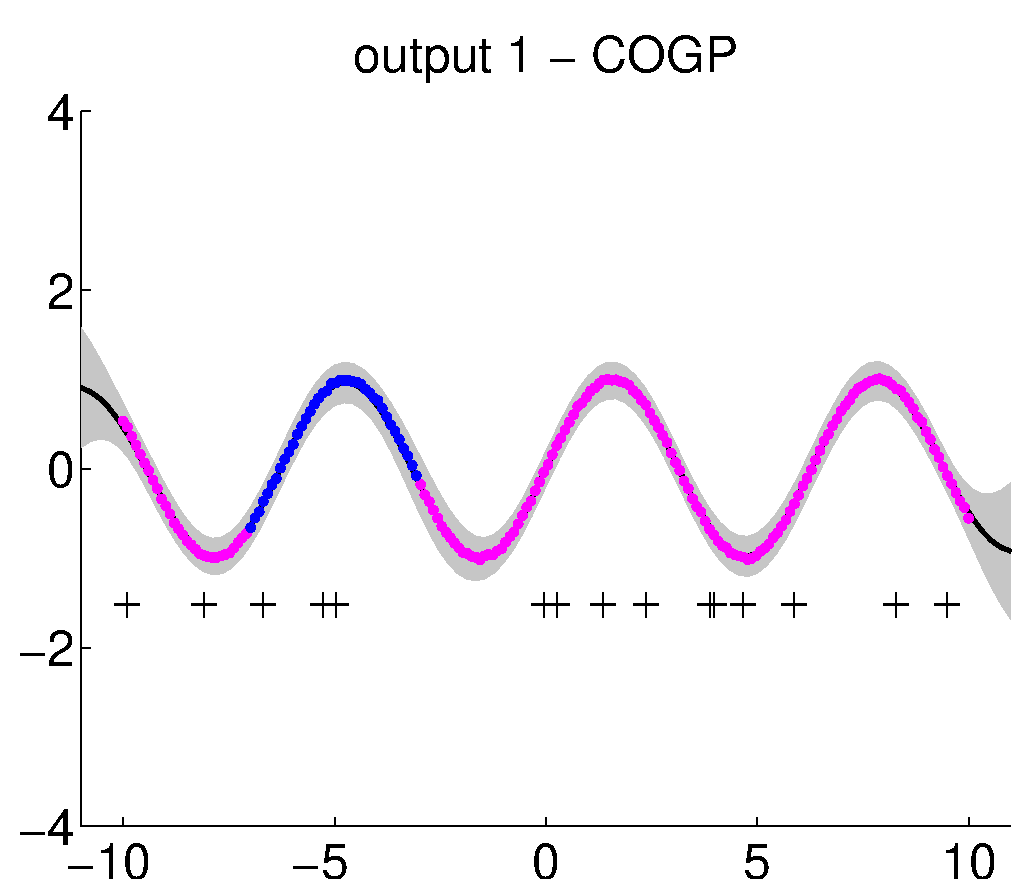
\includegraphics[scale=0.2]{figures/toy-slfm-y1.eps} &
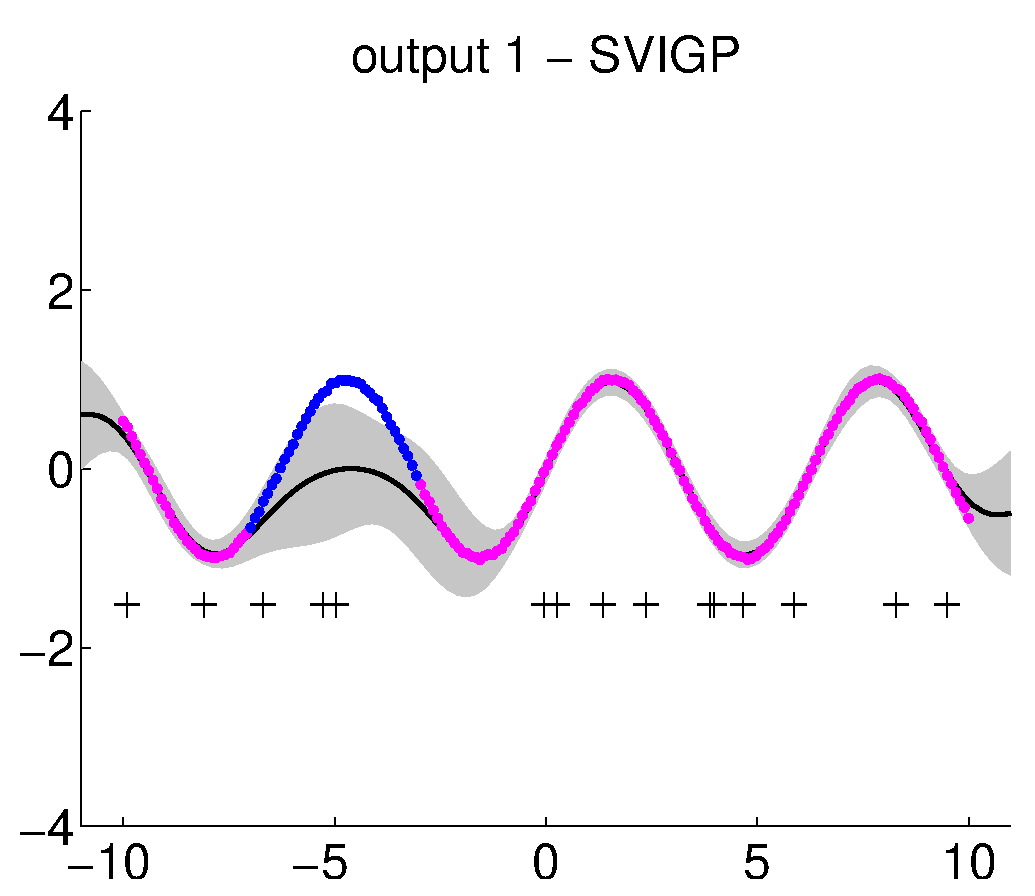
\includegraphics[scale=0.2]{figures/toy-svigp-y1.eps} &
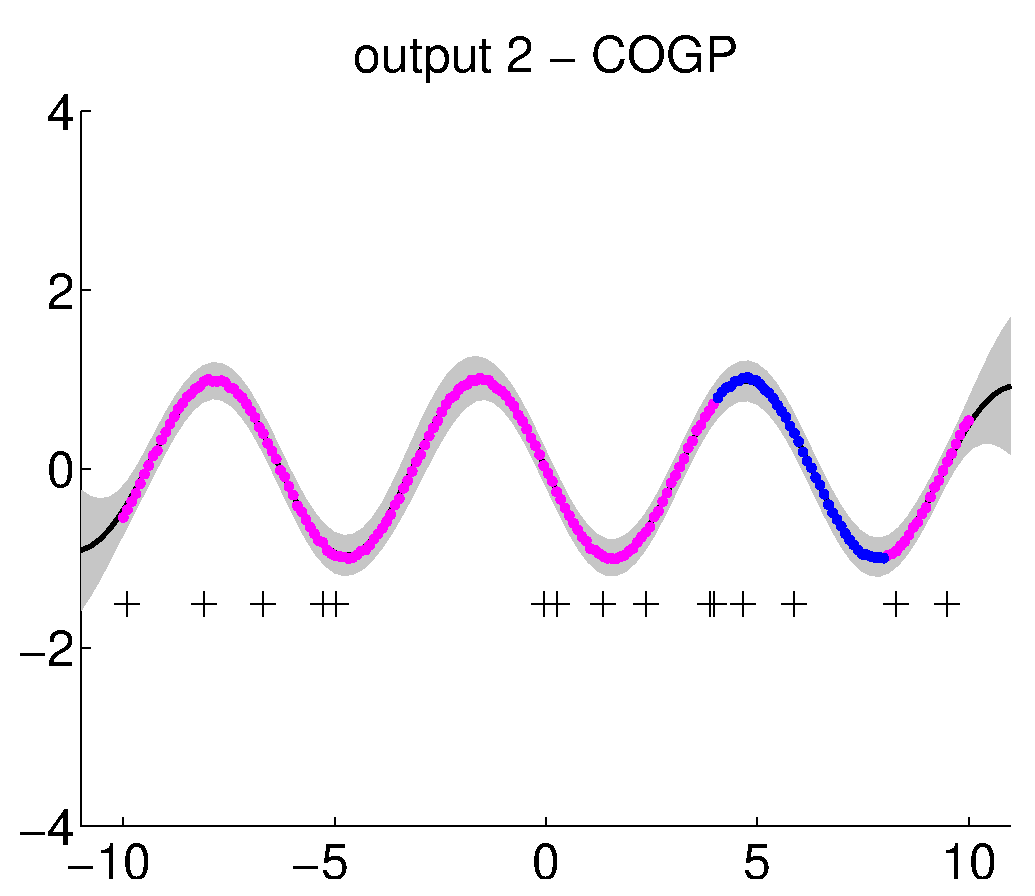
\includegraphics[scale=0.2]{figures/toy-slfm-y2.eps} &
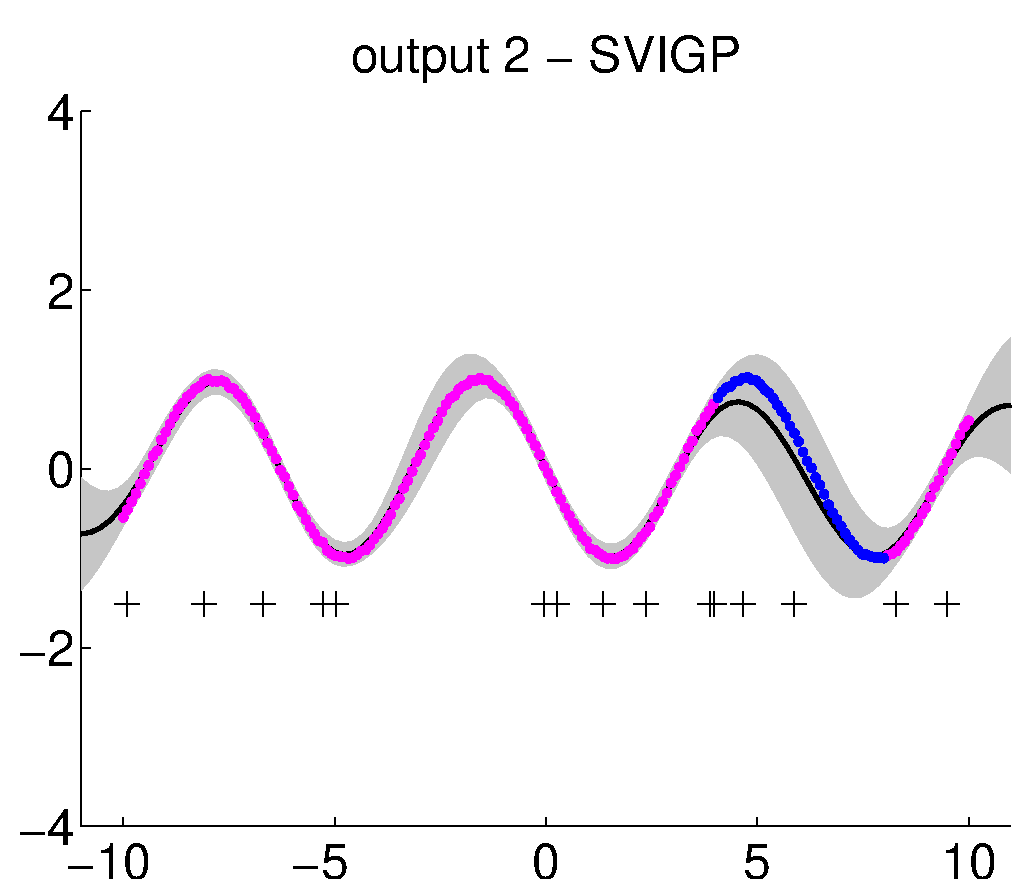
\includegraphics[scale=0.2]{figures/toy-svigp-y2.eps}
\end{tabular}
\caption{Real data and predictive distributions of by COGP (first and third figure) and independent GPs using stochastic variational inference (second and last figure) for the toy problem. Solid black line: predictive mean; grey bar: two standard deviations; magenta dots: real observations; blue dots: missing data. The black crosses show the locations of the inducing inputs. By sharing inducing points across the outputs, COGP accurately interpolates the missing function values.}
\label{fig:toy}
\end{figure*}

\subsection{FOREIGN EXCHANGE RATE PREDICTION}
The first real world application we consider is to predict the foreign exchange rate w.r.t the US dollar of the top 10 international currencies (CAD, EUR, JPY, GBP, CHF, AUD, HKD, NZD, KRW, and MXN) and 3 precious metals (gold, silver, and platinum)\footnote{Data is available at http://fx.sauder.ubc.ca}. 
The setting of our experiment described here is identical to that in \citep{alvarez2010efficient}.
The dataset consists of all the data available for the 251 working days in the year of 2007.
There are 9, 8, and 42 days of missing values  for gold, silver, and platinum, respectively.
We remove from the data the exchange rate of CAD on days 50--100, JPY on day 100--150, and AUD on day 150--200.
Note that these 3 currencies are from very different geographical locations, making the problem more interesting. 
The 153 points are used for testing, and the remaining 3051 data points are used for training.
Since the missing data corresponds to long contiguous sections, the objective here is to evaluate the capacity of the model to impute the missing currency values based on other currencies.
%todo: batch size, learn rate (maybe at the beginning of experiments)

For preprocessing we normalized the outputs to have zero mean and unit variance.
Since the exchange rates are driven by a small number of latent market forces \citep[see e.g.][]{alvarez2010efficient}, we tried different values of $Q = {1,2,3}$ and selected $Q = 2$ which gave the best model evidence (ELBO).
We used the squared-exponential covariance function for the shared processes and the noise covariance function for the individual process of each output.
$M = 100$ inducing inputs (\text{per sparse process}) were randomly selected from the training data and fixed throughout training.

\begin{figure*}
\centering
\begin{tabular}{ccc}
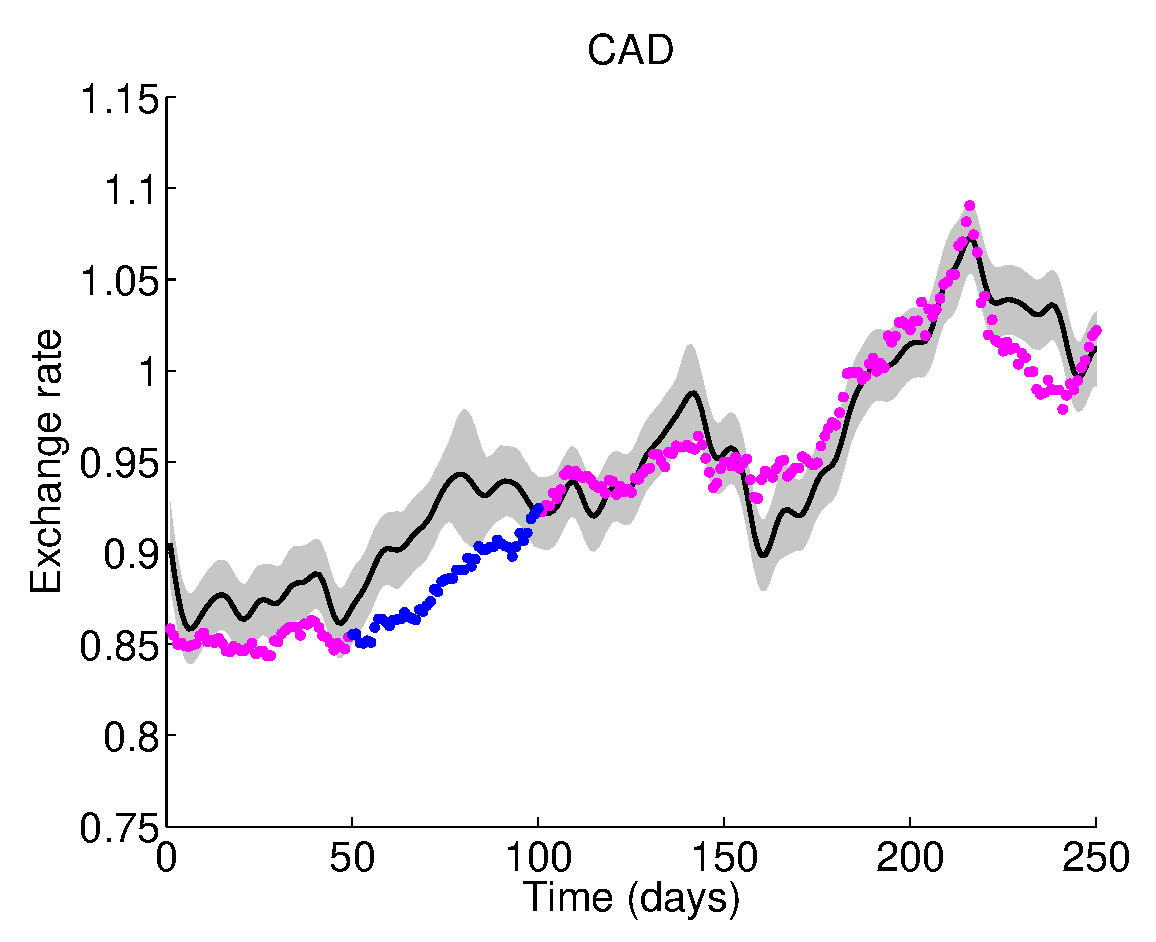
\includegraphics[scale=0.3]{figures/fxCAD.eps} &
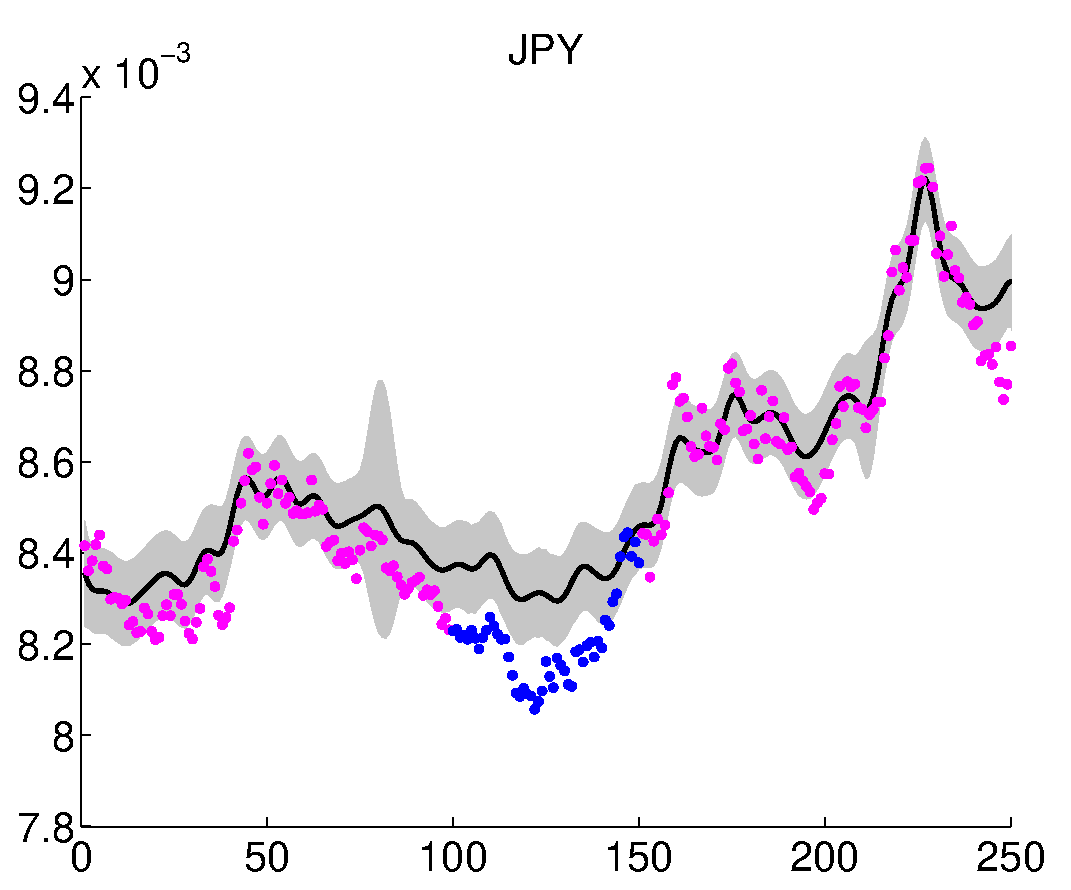
\includegraphics[scale=0.3]{figures/fxJPY.eps} &
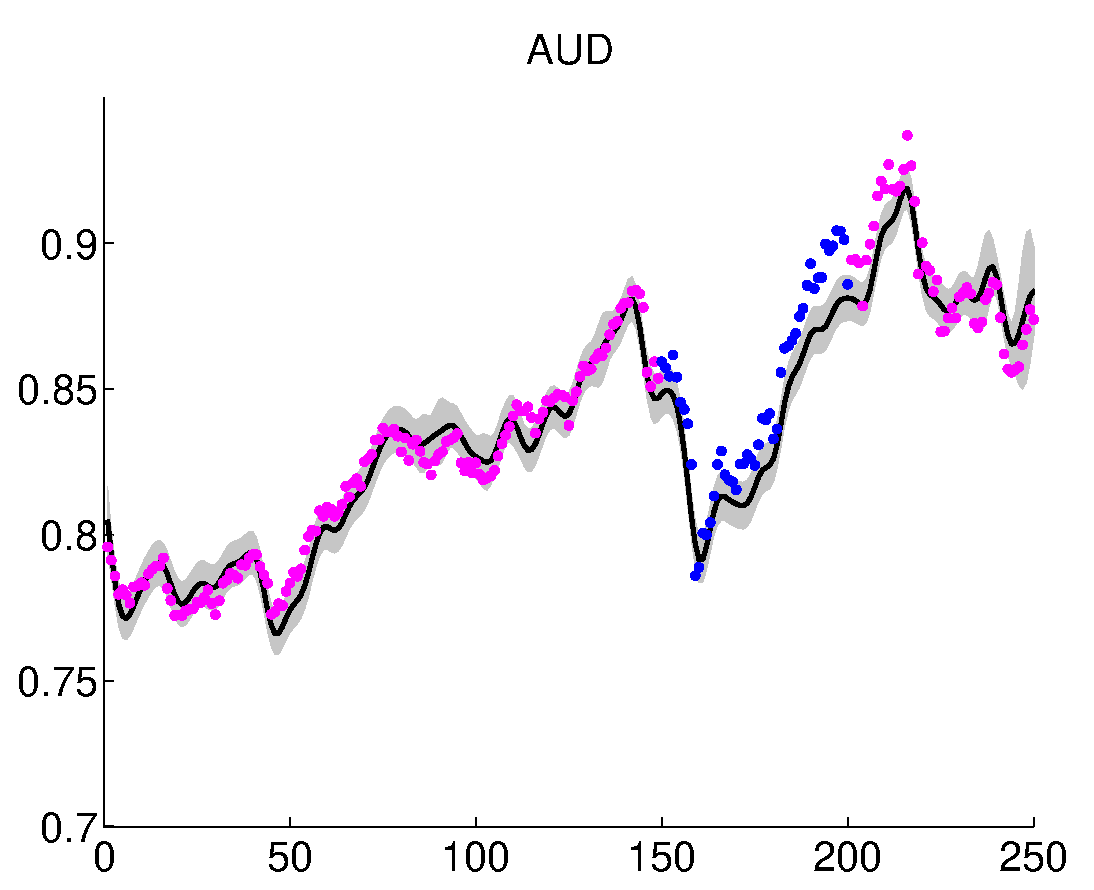
\includegraphics[scale=0.3]{figures/fxAUD.eps}
\end{tabular}
\caption{Real observations and predictive distributions for CAD (left), JPY (middle), and AUD (right). The color coding scheme is the same as in Figure \ref{fig:toy}.}
\label{fig:fx}
\end{figure*}

The real data and predictive distributions by our model are shown in Figure \ref{fig:fx}.
They exhibit similar behaviors to those by the convolved model with inducing kernels in \citet{alvarez2010efficient}.
In particular, both models perform better at capturing the strong depreciation of the AUD than the fluctuations of the CAD and JPY currency.
Further analysis of the dataset found that 4 other currencies (GBP, NZD, KRW, and MXN) also experienced the same trend during the days 
150 -- 200.
This information from these currencies was effectively used by the model to extrapolate the values of the AUD.

%todo: result for independent gps
We also report in Table \ref{tab:fx} the predictive performance of our model compared to the convolved GPs model with exact inference \citep[CGP,][]{alvarez-lawrence-nips-08} and independent GPs (IGP, one for each output).
Our model outperforms both of CGP and IGP in terms of the standardized mean squared error (SMSE).
CGP has lower negative log predictive density (NLPD), mainly due to the less conservative predictive variance of the exact CGP for the CAD currency.
% no std because there are 3 outputs but variance is small
For reference, the convolved GPs with approximation via the variational inducing kernels  \citep[CGPVAR,][]{alvarez2010efficient} has the SMSE of 0.2795 while the NLPD was not provided.
Training took only 10 minutes for our model compared to 1.4 hours for the full CGP model.

\setlength{\tabcolsep}{4pt}
\begin{table}[t]
\caption{Performance comparison on the foreign exchange rate dataset. Results are averages of the 3 outputs over 5 repetitions. Smaller figures are better.}
\label{tab:fx}
\begin{center}
\begin{tabular}{ccc}
\toprule
\textbf{METHOD} & \textbf{SMSE} & \textbf{NLPD} \\ \hline
COGP  & \textbf{0.2125} & -0.8394 \\
CGP & 0.2427 & \textbf{-2.9474} \\
IGP & 0.5996 & 0.4082 \\
%CGPVAR & 0.2795 & NA \\
%ICM & 0.3927 &
\bottomrule
\end{tabular}
\end{center}
\end{table}

\subsection{AIR TEMPERATURE PREDICTION}
Next, we consider the task of predicting air temperature at 4 different locations in the south coast of England. 
The data is gathered from a network of weather sensors (named Bramblemet, Sotonmet, Cambermet, and Chimet), each of which measures several environmental variables \citep{osborne2008towards}\footnote{Data is available at seperate web pages, see e.g. http://www.bramblemet.co.uk}.
%The sensors are close geographically so we can expect correlation in air temperature.
We selected the sensor signal for air temperature during the period from July 10 to July 15, 2013.
The sensors record measurements every 5 minutes, resulting in a maximum of 4320 observations.
There are missing data for Bramblemet (100 points), Chimet (15 points), and Sotonmet (1002 points), possibly due to network outages or hardware failures.
We further simulated failure of the sensors by removing the observations from the time periods [10.2 - 10.8] for Cambermet and [13.5 - 14.2] for Chimet.
The removed data comprises 375 data points and  is used for testing. 
The remaining data consisting of 15,788 points is used for training.
Similar to the previous experiment, the objective is to evaluate the ability of the model to use the signals from the functioning sensors to extrapolate the missing signals.

For pre-processing we normalized the outputs to have zero mean and unit variance.
We used $Q = 2$ sparse processes with the squared exponential covariance function and individual processes with the noise covariance function.
$M=200$  inducing inputs  were randomly selected from the training set and fixed throughout training.
%
\begin{figure*}
\centering
\begin{tabular}{ccc}
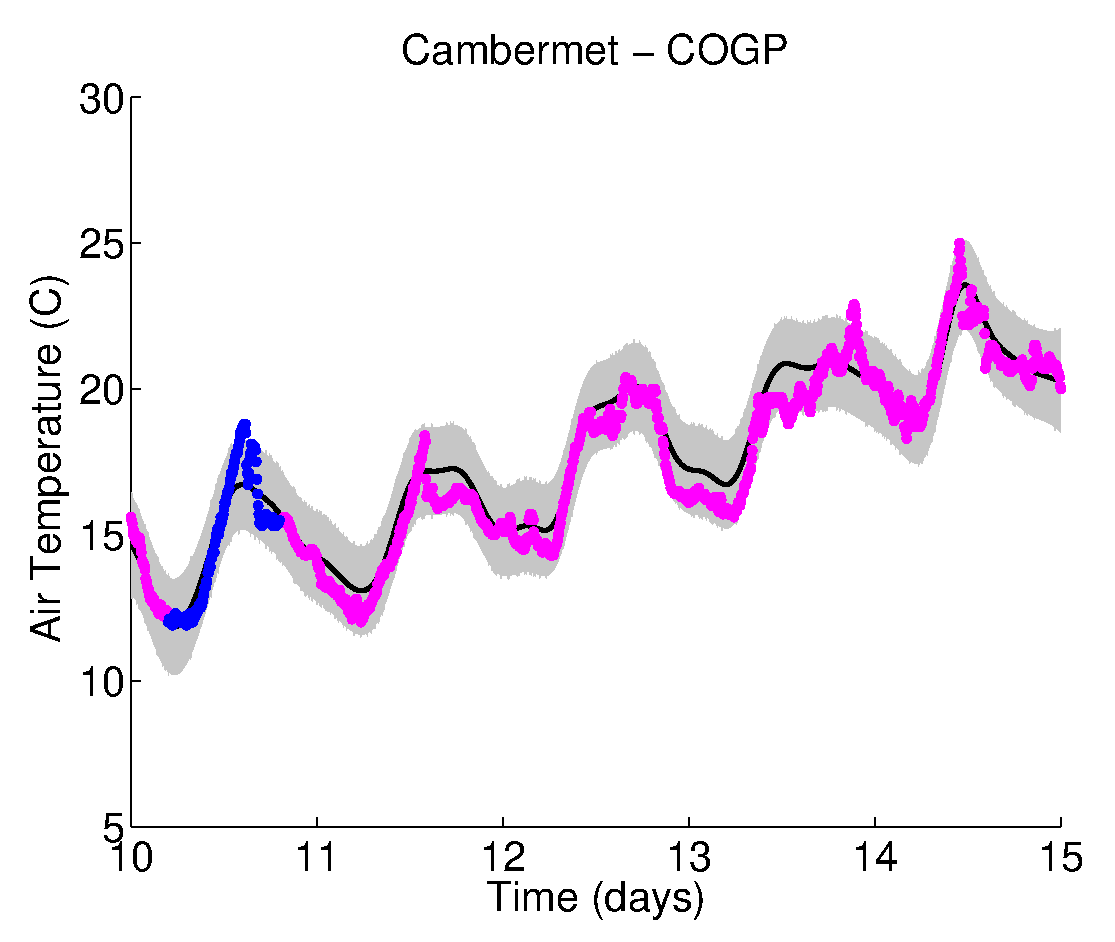
\includegraphics[scale=0.3]{figures/cogp-weatherCambermet.eps} &
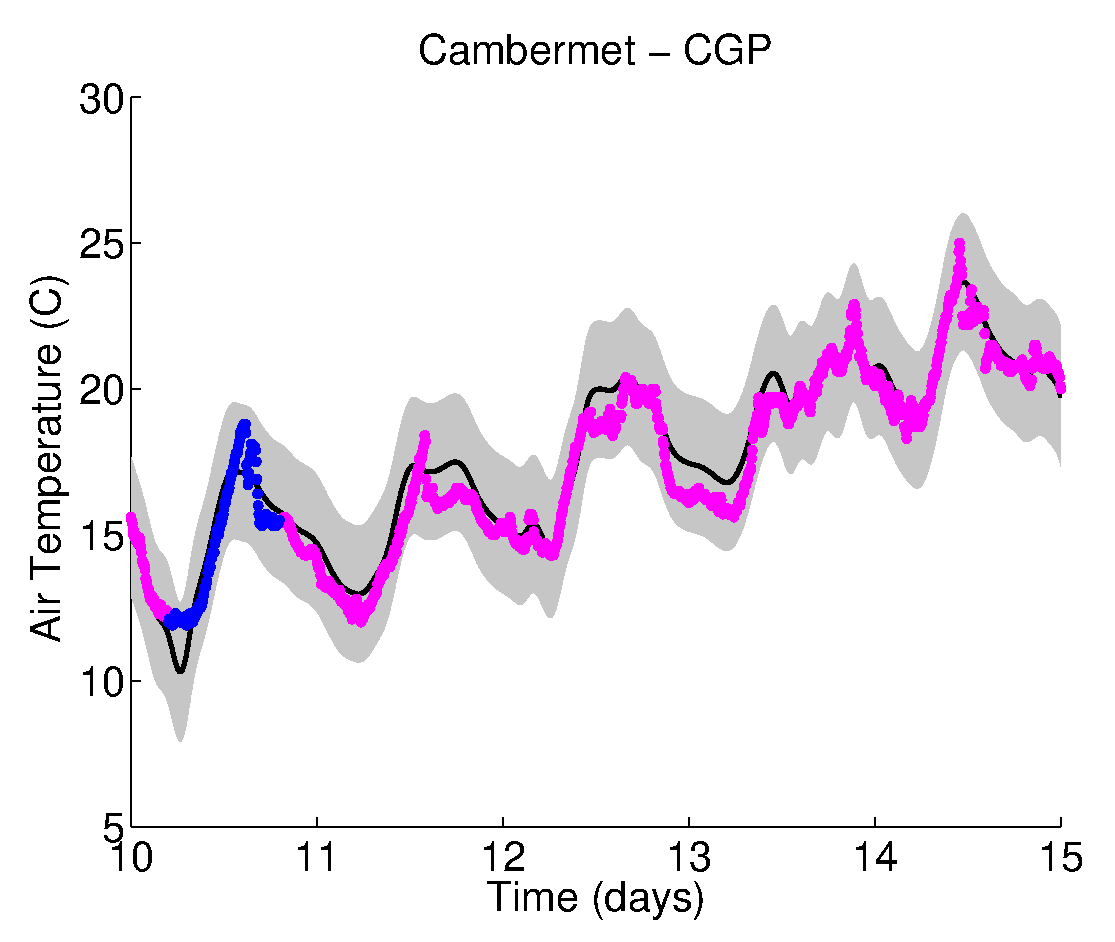
\includegraphics[scale=0.3]{figures/cgp-weatherCambermet.eps} &
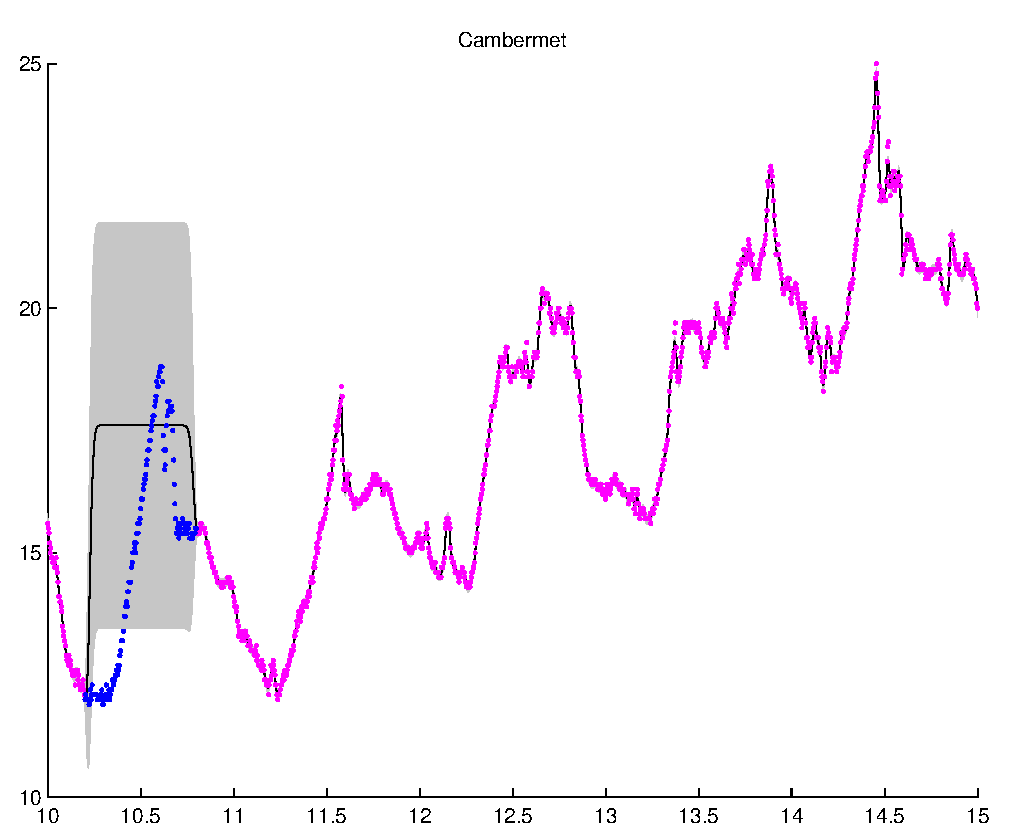
\includegraphics[scale=0.3]{figures/weatherCambermet.eps}
\\
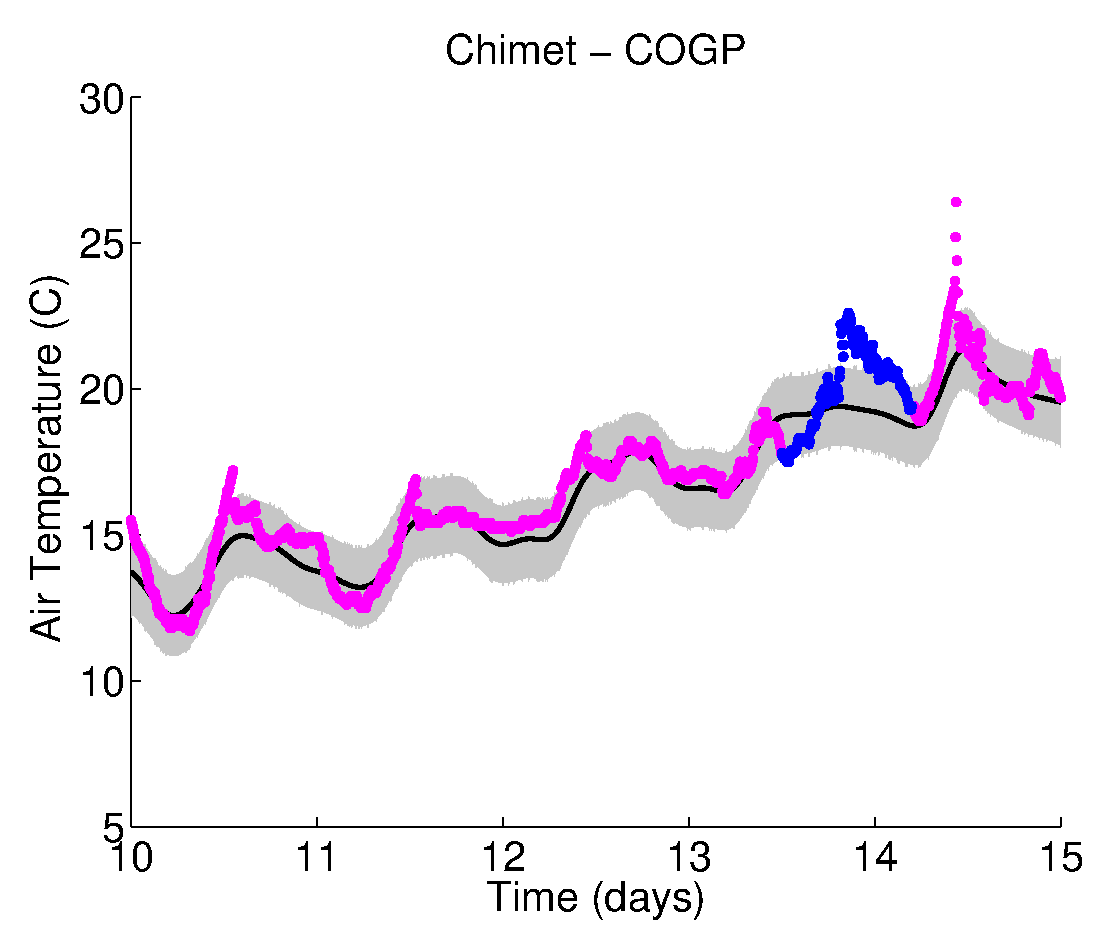
\includegraphics[scale=0.3]{figures/cogp-weatherChimet.eps} &
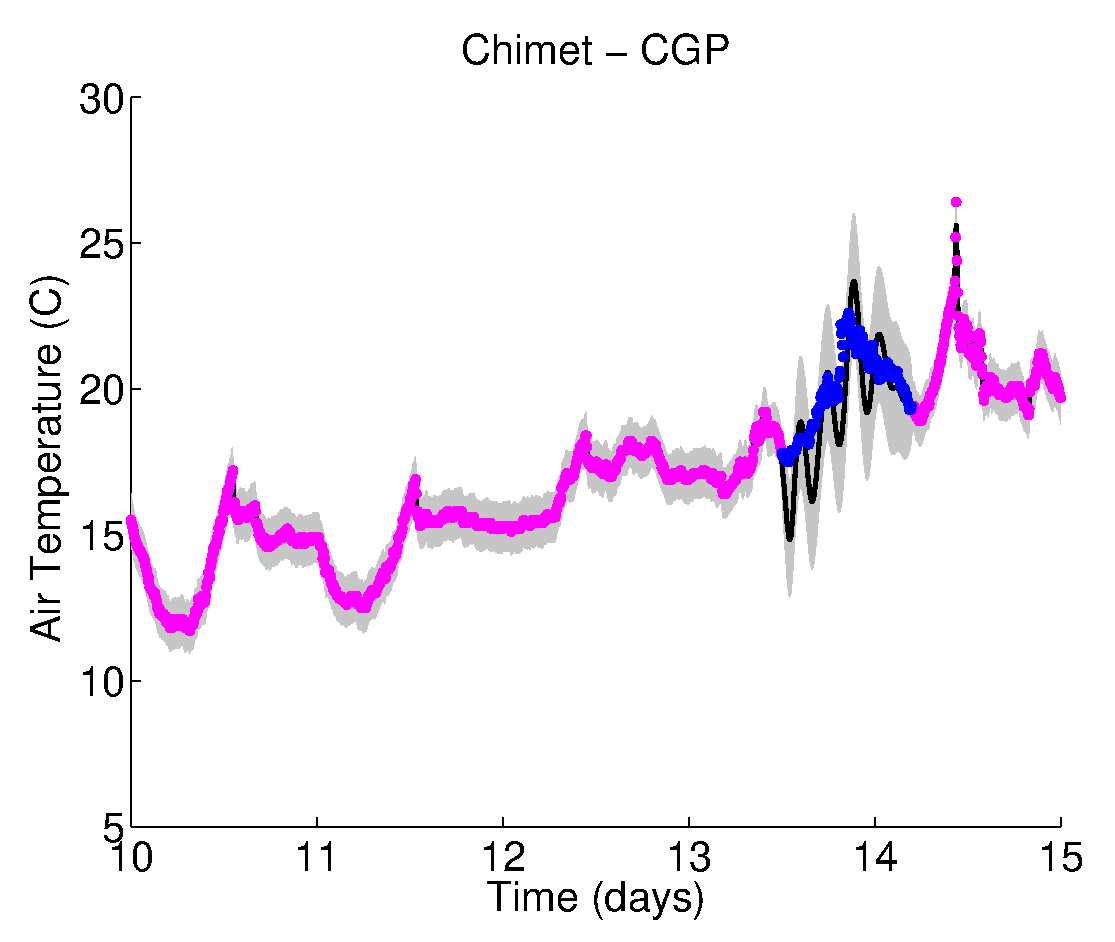
\includegraphics[scale=0.3]{figures/cgp-weatherChimet.eps} &
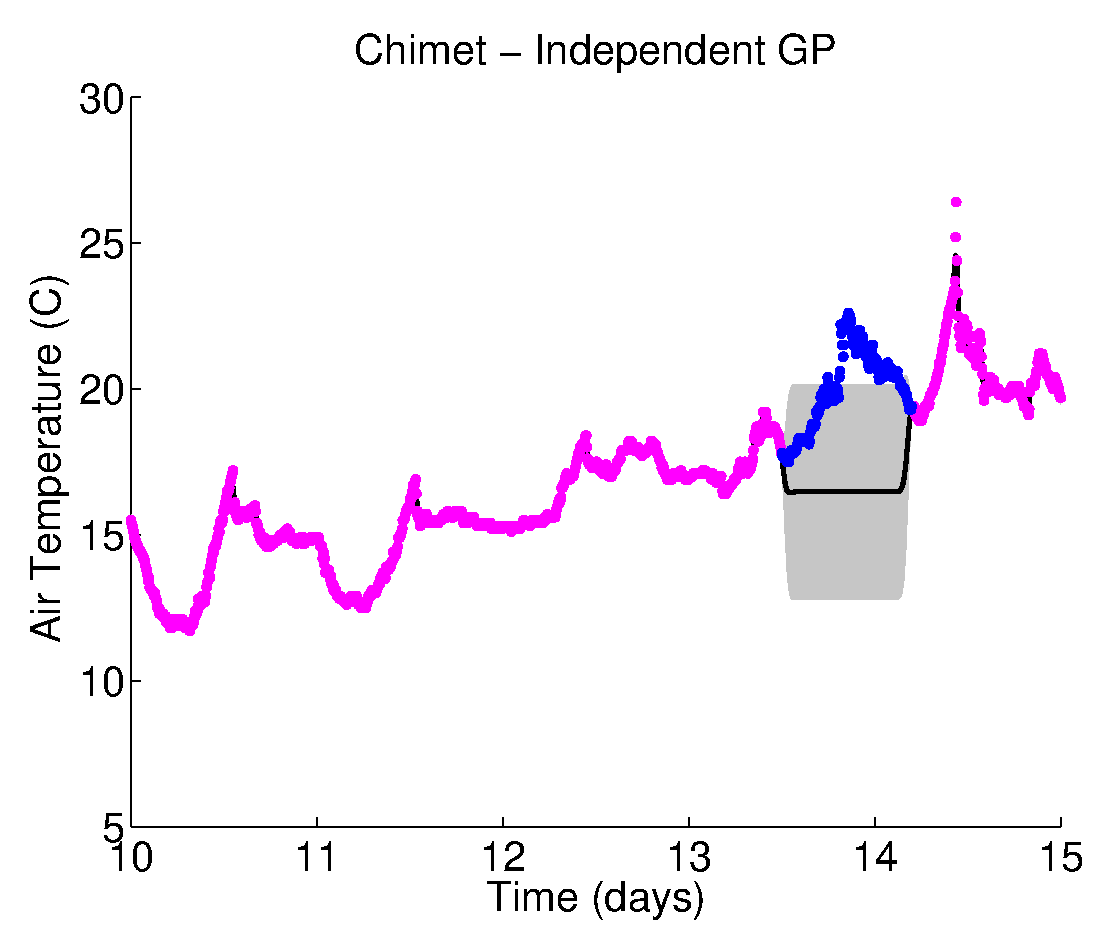
\includegraphics[scale=0.3]{figures/weatherChimet.eps}
\end{tabular}
\caption{Real data and predictive distributions by our method (COGP, left figures), the convolved GP method with exact inference (CGP, middle figures), and full independent GPs (right figures) for the air temperature problem. The coding color scheme is the same as in Figure \ref{fig:toy}.}
\label{fig:weather}
\end{figure*}

The real data and the predictive distributions by our model, CGP with exact inference \citep{alvarez-lawrence-nips-08}, and independent GPs are shown in Figure \ref{fig:weather}.
It is clear that the independent GPs model is clueless in the test regions and thus simply uses the average temperature as its prediction.
For Cambermet, both COGP and CGP can capture the rising in temperature from the morning till the afternoon and the fall afterward.
%For Chimet, both models perform poorly but CGP more so as it falsely predicts  wild fluctuations that are non-existent in the data. 
The comparative performance of the models are summarized in Table \ref{tab:air}, from which it can be seen that our model outperforms CGP in terms of both SMSE and NLPD.
%All results are averaged of the 2 outputs over 5 repetitions.
It took 5 minutes on average to train our model compared to 3 hours of CGP with exact inference.
%
\setlength{\tabcolsep}{4pt}
\begin{table}[t]
\caption{Performance comparison on the air temperature dataset. Results are averages of 2 outputs over 5 repetitions. }
\label{tab:air}
\begin{center}
\begin{tabular}{ccc}
\toprule
\textbf{METHOD} & \textbf{SMSE} & \textbf{NLPD} \\
\hline
COGP & \textbf{0.1077} & \textbf{2.1712} \\
CGP & 0.1125 & 2.2219 \\
IGP & 0.8944 & 12.5319 \\
\bottomrule
\end{tabular}
\end{center}
\end{table}
%
It is also worth noting the characteristics of the sparse processes learned by our model as they indeed correspond to different patterns in the data.
In particular, one process has the inverse lengthscale of 136 which captures the global increase in temperature during the training period while the other has the inverse lengthscale of 0.5 to model the local variations within a single day.

\subsection{ROBOT INVERSE DYNAMICS}
Our last experiment is with a dataset relating to an inverse dynamics model of a 7-degree-of-freedom anthropomorphic robot arm \citep{vijayakumar2000locally}.
The data consists of 48,933 mapping from a 21-dimensional input space (7 joints positions, 7 joint velocities, 7 joint accelerations) to the corresponding 7 joint torques.
%The problem is strongly nonlinear due to complex superpositions of sine and cosine functions in robot dynamics \citep{vijayakumar2000locally}.
%Furthermore, exploratory analysis using standard GP with automatic relevance determination suggests that all of the 21 dimensions are relevant.
It has been used in previous work \citep[see e.g.][]{rasmussen-williams-book,vijayakumar2000locally} but only for single task learning. 
\citet{chai2008multi} considered multitask learning of robot inverse dynamics  but on a different and much smaller dataset.

Here we consider joint learning for the 4th and 7th torques where the first has 2,000 points  while the second has the full data of 44,484 points for training.
The test set consists of 8,898 observations equally divided between the two outputs.
Note that the data was collected at 100Hz for 7.5 minutes in total, hence ideal for this experiment which evaluates the effectiveness of joint learning under the assumption of sparsity in the output spaces.

Since none of the existing multi-output models are applicable to problems of this scale, we compare with independent models that learn each output separately.
Standard GP is applied to the first output as it has only 2,000 observations for training.
For the second output, we used two baselines.
The first is the subset of data (SOD) approach where 2,000 data points are randomly selected for training with a standard GP model.
The second is the sparse GP with stochastic variational inference (SVIGP) using 500 inducing inputs and a batch size of 1,000.
In case of COGP, we also used a batch size of 1,000 and 500 inducing points for the shared process ($Q = 1$) and each of the individual processes.
The squared exponential with automatic relevance determination (SEard) covariance function is used for all processes of all methods.
Finally, the outputs are normalized to have zero mean and unit variance. 

\begin{table}[t]
\caption{Performance comparison on the robot inverse dynamics dataset. In the last two lines, standard GP is applied to output 1 and the other method is applied to output 2. Results are averaged over 5 repetitions. }
\label{tab:robotarm}
\begin{center}
\begin{tabular}{lcccc}
\toprule
& \multicolumn{2}{c}{\textbf{OUTPUT 1}} & \multicolumn{2}{c}{\textbf{OUTPUT 2}} \\ \cmidrule(r){2-5}
\textbf{METHOD} & \textbf{SMSE} & \textbf{NLPD} & \textbf{SMSE} & \textbf{NLPD}\\ 
 \midrule
COGP, learn z & \textbf{0.2631} & \textbf{3.0600} & 0.0127 & \textbf{0.8302} \\
COGP, fix z & 0.2821& 3.2281 & 0.0131 & 0.8685 \\
GP, SVIGP & 0.3119 & 3.2198 & \textbf{0.0101} & 1.1914 \\
GP, SOD & 0.3119 & 3.2198 & 0.0104 & 1.9407 \\
\bottomrule
\end{tabular}
\end{center}
\end{table}

The performance of all methods in terms of SMSE and NLPD is given in Table \ref{tab:robotarm}.
The benefits of learning the two outputs jointly are evident, as can be seen by the significantly lower SMSE and NLPD of COGP compared to the full GP for the first output (4th torque).
While the SMSE of the second output is essentially the same for all methods, the NLPD of COGP is substantially better than that of the independent SVIGP model which has the same amount of training data for this torque.
The results validate the impact of collaborative learning even when under sparsity assumption, thus open up new opportunities for improvement over single task learning with independent sparse processes.

% table for smses, nlpds, training tiem
\begin{figure}
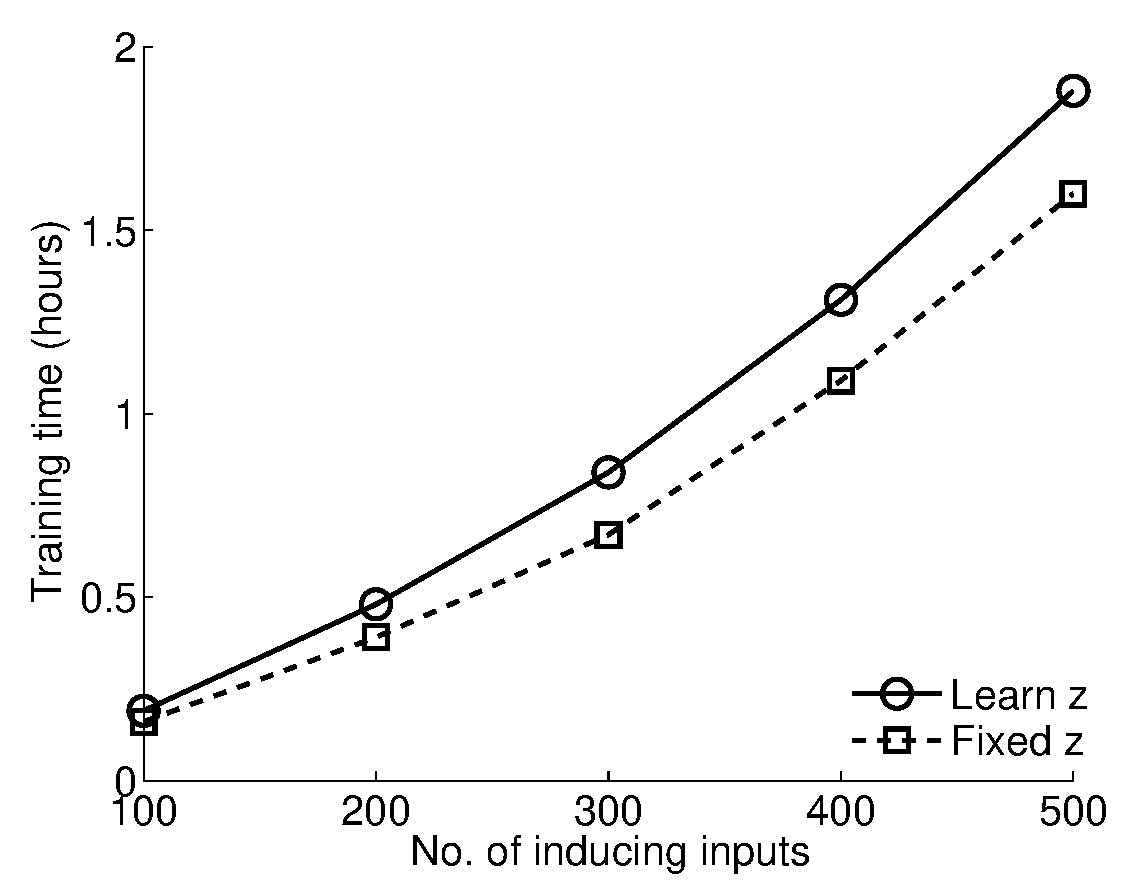
\includegraphics[scale=0.4]{figures/sarcosTime.eps}
\caption{The cost of optimizing versus fixing the inducing inputs.}
\label{fig:time}
\end{figure}

Also from Table \ref{tab:robotarm}, we see that optimizing the inducing inputs can lead to better performance than fixing them.
More importantly, the overhead in computation is small, as demonstrated by the training time using the two options in Figure \ref{fig:time}.
For instance, the total training time is only 1.9 hours when learning with 500 inducing inputs compared to 1.6 hours when fixing them.
As this dataset is 21-dimensional, the small difference in training time confirms that learning of the inducing inputs is a practical option even when dealing with problems of high dimensions.
%As this dataset is 21-dimensional, the small difference in training time our analysis that the cost of optimizing the inducing inputs only scales sublinearly with the dimensionality of the problem.
%Thus, for datasets of high dimension, learning of the inducing inputs is a practical option.


\section{DISCUSSION}
We have presented scalable multi-output GPs for learning of correlated functions.
The formulation around the inducing variables and their encapsulation of sufficient statistics was shown to be conducive to not only effective but also scalable joint learning under sparsity. 
We note that although our large scale experiment was done with over 40,000 observations -- the largest publicly available multi-output dataset we could find, the model can easily handle much bigger datasets.

We discuss several interesting extensions to this work.
First, consider the model for the single GP case, i.e., $P = 1$. By using $Q > 1$ sparse processes, the GP can now have multiple set of inducing variables.
These can be made local to capture varying characteristics of the latent process in different  input regions, for e.g. similar to the 
work by \citet{nguyen2014fast}, leading to scalable GPs with non-stationary properties. 

A further extension is to replace the constant mixing weights in the model with input-dependent coefficients as in the Gaussian process regression networks framework \citep[GPRN,][]{wilson-et-al-icml-12} to accommodate adaptive dependencies among the outputs.
We leave  these extensions to future work.

%\subsubsection*{Acknowledgements}

\bibliographystyle{plainnat}
\bibliography{references}

\end{document}
